% SpareCycles final report. Build: make report (or upload docs/report/ to Overleaf).
\documentclass[conference]{IEEEtran}

\usepackage{cite}
\usepackage{amsmath,amssymb}
\usepackage{graphicx}
\usepackage{booktabs}
\usepackage{xcolor}
\usepackage{listings}
\usepackage{pgfplots}
\usepackage{url}
\usepackage[hidelinks]{hyperref}
\pgfplotsset{compat=1.18}

% Let floats fill more of a page, so that figures stay near their section
% instead of collecting after the references.
\renewcommand{\topfraction}{0.9}
\renewcommand{\dbltopfraction}{0.9}
\renewcommand{\bottomfraction}{0.8}
\renewcommand{\textfraction}{0.07}
\renewcommand{\floatpagefraction}{0.6}
\renewcommand{\dblfloatpagefraction}{0.6}
\setcounter{topnumber}{3}
\setcounter{dbltopnumber}{3}
\setcounter{totalnumber}{5}

% Marks text that an owner still has to write. Remove all of them before submission.
\newcommand{\todo}[1]{\textcolor{red}{[TODO: #1]}}

\lstset{basicstyle=\ttfamily\scriptsize, columns=fullflexible, breaklines=true, frame=single, xleftmargin=2pt, xrightmargin=2pt}
\graphicspath{{diagrams/}{screenshots/}}

\begin{document}

\title{SpareCycles: A Fault-Tolerant Volunteer Computing Platform}

\author{
\IEEEauthorblockN{Tejas Chakkarwar}
\IEEEauthorblockA{Student ID: \todo{ID}\\ \todo{email}}
\and
\IEEEauthorblockN{Kushagra Bainsla}
\IEEEauthorblockA{Student ID: 019016061\\ kushagra.bainsla@sjsu.edu}
\and
\IEEEauthorblockN{Abhishek Ahirrao}
\IEEEauthorblockA{Student ID: \todo{ID}\\ \todo{email}}
}

\maketitle

\begin{abstract}
Volunteer computing harnesses idle machines for large computations, but volunteers can leave at any moment or return wrong results, and the coordinator that distributes the work is a single point of failure. We present SpareCycles, a volunteer computing platform in Go and gRPC that tolerates all three faults. Volunteers pull work units from a leader under leases, so lost units are reassigned. Each unit runs on three volunteers and is accepted by majority vote, and resource discovery assigns units using reported resources and a trust score learned from the votes. Three coordinators elect a leader with the Bully algorithm extended with terms and a majority lease, and replicate every task-table change to a backup before it takes effect. SWIM gossip detects failed members, and tokens and signed tasks secure the system. On a local cluster, a crashed volunteer was declared dead in 2.9\,s, a faulty volunteer was outvoted and blocked, and a new leader took over 2.5\,s after a crash without losing accepted work. Majority voting costs 32\% of throughput with four volunteers.
\end{abstract}

% Section 2. Owner: Tejas. Sources: docs/proposal.md sections 1-2, site/index.html.
\section{Project Goals and Motivation}
\label{sec:goals}

Many computations in science and engineering are embarrassingly parallel: a large job can be cut into many pieces that never need to talk to each other. SpareCycles runs such jobs on donated machines. A client submits a job, a coordinator splits it into work units, which the design sizes at about 60 seconds each, volunteer computers pull the units, run them and return the results, and the coordinator merges the accepted results into the final output. What makes this hard is that every participant except the client may misbehave. A volunteer can disappear at any moment because its owner closes a laptop or a spot instance is reclaimed. It can return a wrong result, through faulty hardware or on purpose. And the coordinator itself can crash, taking with it the only record of which units are finished.

Most personal computers are idle for a large part of the day, and projects such as SETI@home and Folding@home have shown that this idle capacity can carry real research. Anderson estimates that buying the throughput of a typical large BOINC project on Amazon EC2 would cost about 420 times as much as running the project on volunteer machines~\cite{anderson2020boinc}. The same setting is also a demanding distributed system. The machines are anonymous and untrusted, their hardware and speed differ widely, they join and leave continuously, failures are the normal case rather than the exception, and some participants may be malicious. A platform for students and researchers must handle all of these problems at once, with a small operating budget.

We therefore set the following goals. First, a job must produce the correct result although volunteers leave or crash while they hold work. Second, it must produce the correct result although some volunteers return wrong results, by accident or by design. Third, the platform must have no single point of failure: when the coordinator that assigns work fails, another one must take over and continue the job without losing accepted work. Fourth, the system must run on AWS EC2, with three coordinators in different availability zones and volunteers on spot instances, on-demand instances and our own laptops, and every mechanism must be observable through metrics and logs. We implement all distributed algorithms ourselves.

Not every job fits this model. A suitable job splits into units that are independent, so that they can run in any order on any machine; deterministic, so that two honest volunteers return identical bytes that can be compared by hash; and compute-heavy relative to their input and output, so that shipping a unit costs far less than running it. Fractal image tiles and Monte Carlo sampling, our two workloads, have all three properties. Tightly coupled computations whose pieces exchange data, jobs that need low latency, jobs that move large data sets per unit, and computations whose results legitimately differ from one processor to another do not fit unless they are restructured.

% Section 3. Owner: Abhishek. Sources: docs/proposal.md section 2, AGENTS.md design decisions.
\section{Distributed Systems Challenges Addressed}
\label{sec:challenges}

Volunteer computing brings several classic problems of distributed systems together in one setting. The machines that do the work are outside the operator's control, they join and leave at will, and the coordinator that tracks the work is itself a machine that can fail. SpareCycles addresses the following challenges, each with a dedicated mechanism that Section~\ref{sec:design} describes in detail.

\begin{itemize}
\item \emph{Volunteer churn.} A volunteer can stop at any moment and take its work unit with it. Every unit is handed out under a lease, and SWIM gossip detects a crashed volunteer within seconds, so the leader releases its leases long before they would expire.
\item \emph{Incorrect results.} A volunteer can return a wrong result through faulty hardware or on purpose. Each unit runs on three different volunteers and is accepted only when two results agree. Volunteers whose results lose votes lose trust, and below a threshold they receive no more work.
\item \emph{Coordinator failure.} A single coordinator, like BOINC's project server, is a single point of failure. SpareCycles runs three coordinators that elect a leader with the Bully algorithm, so a backup takes over when the leader crashes.
\item \emph{Split brain.} A timeout cannot tell a crashed leader from an unreachable one, so plain Bully can produce two leaders that both hand out work. Every election therefore starts a new term, nodes reject messages from older terms, and a leader may act only while 2 of 3 coordinators have recently confirmed it (a leader lease).
\item \emph{State loss on failover.} A new leader is of little use if it does not know which units were assigned and accepted. Every change to the task table reaches a backup before it takes effect, and a new leader loads the newest replicated table before it serves any request.
\item \emph{Heterogeneity.} Volunteers differ in cores, memory and speed. Resource discovery matches units to volunteers on their reported resources and their trust, so that slow volunteers do not hold up the oldest jobs.
\item \emph{Untrusted participants.} Anyone could pose as a volunteer, or as a coordinator handing out tasks. Volunteers authenticate with per-volunteer tokens and per-session secrets, and the leader signs every task, so a volunteer runs only work that the leader issued.
\end{itemize}

% Section 4. Owners: Tejas (BOINC), Kushagra (SWIM, VECA), Abhishek (Bully, VECTrust).
\section{Literature Review}
\label{sec:literature}

\subsection{Volunteer Computing with BOINC}
\todo{Tejas, about 0.8 page, on \cite{anderson2004boinc} and \cite{anderson2020boinc}: the project server model, work units and replication, result validation by comparing replicas (and its homogeneous redundancy for floating-point results), credit, and the central server as a single point of failure. End with what SpareCycles takes from BOINC and what it changes.}

\subsection{Group Membership and Failure Detection: SWIM}
Large distributed systems need every member to learn, quickly and at low cost, that another member has failed. The classic approach, in which every member periodically sends a heartbeat to every other member, produces a network load that grows quadratically with the group size, and either detection time or false-positive rate degrades as the group grows. Das, Gupta and Motivala~\cite{das2002swim} address this with SWIM, whose central idea is to separate \emph{failure detection} from the \emph{dissemination} of membership updates.

For detection, each member runs a protocol period of fixed length. In every period it picks one other member and sends it a \textit{ping}. If no acknowledgement arrives within a timeout, it does not declare the member failed; instead, it asks $k$ other members to probe the target on its behalf with a \textit{ping-req}. Only if none of these indirect probes succeeds is the target considered failed. The indirect probes make the detector robust to a single congested or lossy link between two healthy members, and the authors show that the probability of a false positive falls quickly as $k$ grows. Because each member sends a constant number of messages per period, the load per member is independent of the group size, and the expected time until some member first detects a failure is a constant number of protocol periods, $e/(e-1)$, also independent of the group size.

For dissemination, SWIM does not broadcast. Membership updates are \emph{piggybacked} on the ping, ping-req and acknowledgement messages that the detector already sends, so they spread in the manner of an epidemic, reaching the whole group in a number of periods that grows only logarithmically with its size, at no extra message cost.

The paper adds two refinements that our implementation adopts. First, a \emph{suspicion} subprotocol: a member that does not answer is first marked \textit{suspect} rather than dead, and the suspicion is gossiped to the group. If the suspected member is alive, it learns of the suspicion and refutes it by announcing itself alive with a higher \emph{incarnation number}; only a suspicion that survives a timeout becomes a confirmed failure. Incarnation numbers give a precedence order between conflicting updates about the same member, which keeps the protocol consistent without coordination. Second, probe targets are chosen in a randomly shuffled \emph{round-robin} order rather than uniformly at random, which bounds the worst-case time until a failed member is probed by some member to a number of periods linear in the group size.

SWIM is a natural fit for volunteer computing. Volunteers join and leave continuously, the group can grow large, and a coordinator that relies on lease expiry alone learns of a crash only after a full lease, which for our 60-second units is three minutes. With SWIM, the coordinator learns of the crash within seconds and reassigns the lost work early (Section~\ref{sec:scenario-volunteer}).

\subsection{Volunteer Edge-Cloud Computing: VECA}
Yeddulapalli et~al.~\cite{yeddulapalli2024veca} study volunteer edge-cloud computing, in which individuals and organizations contribute laptops, desktops and servers to run machine-learning and deep-learning workflows. They identify two obstacles: the nodes are intermittent and volatile, which makes workflow performance unpredictable, and the owners of the nodes must not see the workflow's models and data. Their framework, VECA, makes a three-fold contribution.

The first is \emph{capacity-based clustering}: nodes are grouped with $k$-means on their number of CPUs, memory and storage, and the clustering is repeated when the number of nodes grows by 10\%, so that a scheduler searches one suitable cluster instead of all nodes. The second is a \emph{two-phase scheduler}. A cloud hub first selects the cluster whose capacity best matches the workflow; an agent in that cluster then uses a recurrent neural network to forecast each node's probability of being online, ranks the nodes, and schedules on nodes whose predicted availability is at least 0.8, preferring the one nearest the user. If the chosen node fails, a fail-over step reads the stored workflow details and the precomputed node order from a Redis cache and resumes execution on the next node, without running the forecasting model again. The third is \emph{confidential computing}: confidential workflows run only on nodes that support AWS Nitro Enclaves, using an encrypted image, isolated CPU and memory, and an attestation document that proves the enclave's identity.

VECA was implemented with OpenFaaS, MicroK8s and Docker and evaluated in simulation with 50 nodes in four clusters, synthetic availability traces and two scientific workflows. It reports a two-fold reduction in node search latency over the next best approach and a mean productivity rate (the share of execution time not spent on recovery) of 86.9\%, against 66.7\% and 65.7\% for two earlier frameworks.

VECA and SpareCycles address the same root problem, volatile volunteer nodes, from opposite directions. VECA tries to \emph{avoid} failures by predicting availability and placing work on nodes that are likely to stay online, and it recovers by fail-over to the next node. SpareCycles assumes that failures and even malicious nodes are normal: it \emph{detects} failures by gossip, \emph{recovers} through leases and reassignment, and \emph{tolerates} incorrect results through replication and voting, in the BOINC tradition. VECA's availability forecasting would complement our resource discovery (Section~\ref{sec:design}), and its use of enclaves addresses a confidentiality requirement that SpareCycles deliberately leaves out of scope: our workloads are public scientific computations, and we protect the \emph{integrity} of tasks with signatures rather than their confidentiality.

\subsection{Leader Election: the Bully Algorithm}
\todo{Abhishek, about 0.4 page, on \cite{garciamolina1982elections}: assumptions (synchronous system, failure detection by timeout), the election, answer and coordinator messages, the highest live identifier wins, message complexity (worst case quadratic), and why it is unsafe under network partitions. Explain how term numbers and a majority leader lease fix this in SpareCycles.}

\subsection{Trusted Resource Allocation: VECTrust}
\todo{Abhishek, about 0.4 page, on \cite{pandey2021vectrust}: how VECTrust computes trust for volunteer resources and uses it in allocation, its evaluation, and how SpareCycles' resource discovery (trust scores updated from voting) builds on it.}

% Section 5. Owners: 5.1 split; 5.2 each person for own algorithms; 5.3 text Abhishek; diagrams per docs/report/outline.md.
\section{Project Design}
\label{sec:design}

\subsection{Design Goals}
\label{sec:design-goals}

\paragraph{Heterogeneity, quality of service, scalability}
Volunteers differ in processor, memory and speed, and the coordinator cannot inspect them. Each volunteer therefore reports its CPU cores, memory and a speed score when it registers. Resource discovery uses the reported memory and speed (the cores are recorded but not used) together with a trust score learned from past votes: a volunteer that reports less than the configured minimum memory gets no units, a slow volunteer takes the newest units and leaves the end of a job to faster ones, and a volunteer with a poor record is kept away from deciding copies or blocked. Heterogeneity also threatens voting, since different processors can round floating-point operations differently. Rather than restrict votes to identical hardware, as BOINC's homogeneous redundancy does, we require every workload to return identical bytes on every architecture: the Monte Carlo workload uses only integer arithmetic, and the fractal workload rounds every product explicitly so that the compiler cannot fuse a multiply and an add on one architecture but not on another. Quality of service comes from bounding how long a unit can be held up. A lease bounds the wait for a lost unit to three minutes, and gossip usually shortens it to seconds; because a unit is accepted as soon as two of its three copies agree, one slow copy does not delay it. Scalability rests on two choices. Volunteers pull work, so the leader keeps no queue per volunteer and an idle volunteer costs one request per second, and gossip costs each member a constant number of messages per period, whatever the size of the group. Every table change still passes through the single leader, which is why the design targets units of about a minute: each unit then costs the leader only a few table changes (three assignments, up to three results and one acceptance) for several minutes of volunteer computation.

\paragraph{Openness}
All interaction happens through a single, versioned gRPC contract (Section~\ref{sec:components}). Any program that speaks this protocol can act as a client or a volunteer, and new workloads are added by implementing three functions (split, run, merge) without changing the coordinator. Every internal mechanism is a small Go interface with interchangeable implementations, so a team member can replace an algorithm without touching the rest of the system.

\paragraph{Security}
Volunteer computing gives work to machines that the operator does not control, so the coordinator must decide who may join and each volunteer must be able to tell a genuine task from a forged one. SpareCycles authenticates volunteers with per-volunteer tokens at registration and signs every task it hands out. A signature binds the task's payload to its unit, workload and lease expiry, so a captured task cannot be replayed for another unit or after its lease. Integrity of results, which a volunteer can still falsify, is protected separately by majority voting. Confidentiality of task data is out of scope (Section~\ref{sec:literature}).

\paragraph{Failure handling}
We treat failure as the normal case. A volunteer may stop at any moment; SWIM gossip declares it dead within seconds and the leader immediately releases its leases, while lease expiry remains as a slower safety net for volunteers that cannot take part in gossip. Every change to the task table is replicated before it takes effect, so a new leader can continue a job after the old one crashes. Faults are also contained: a volunteer that receives a task with a bad signature stops at once rather than taking more units it will never complete.

\paragraph{Concurrency, transparency}
A coordinator serves many volunteers and clients at the same time, and gRPC runs each request in its own goroutine, so all shared state must be guarded. The design keeps the number of possible orderings small. Every change to the task table passes through a single commit path that validates, replicates and applies it under one mutex, so the leader's changes form one total order, which is also the order in which the backups apply them. Recording a result and voting on its unit happen together under a second lock, so two results that arrive at the same moment yield one decision rather than two. The remaining shared state, such as the volunteer list, session hashes, trust scores and the election and gossip state, is protected by a mutex inside its own component, and the continuous integration pipeline runs every test with Go's race detector.

Transparency means that clients and volunteers never need to know which coordinator leads, or whether a failover has happened. They hold a connection to all three coordinators and send each call to the one that answered last. A follower answers \texttt{FAILED\_PRECONDITION} and a crashed node is \texttt{UNAVAILABLE}; in both cases the call moves on to the next coordinator (\texttt{leaderclient}). Replication is equally invisible: a job is confirmed only after its change is on two coordinators, so a client that polls a new leader finds its job where it left it. The only visible effect of a failover is that volunteers register again, because session secrets are deliberately kept on the leader alone.

\subsection{Key Components and Algorithms}
\label{sec:algorithms}

The system has three roles. \emph{Clients} submit jobs and fetch results. \emph{Coordinators}, three in total, hold the task table; one is the leader and the others are backups. \emph{Volunteers} pull work from the leader, run it and return results. Six algorithms from the course list work together:

\paragraph{Leases and reassignment (resource allocation)} When a volunteer pulls a unit, the leader records an assignment whose lease expires a fixed time later (\texttt{SC\_LEASE\_DURATION}, by default three minutes, three times the 60-second unit the design targets). The expiry is stored in the replicated task table and included in the signed task, and the volunteer cancels its own computation when the expiry passes. Once per second the leader asks the \texttt{lease.Timeout} policy for every lease in an open unit whose expiry has passed, and commits a \texttt{LeaseReleased} change for each; the unit then needs a volunteer again and goes to the next one that asks (Fig.~\ref{fig:unit-state}). A result is recorded only from a volunteer that still holds a lease on the unit, so a volunteer that lost its lease cannot complete the unit afterwards. Gossip normally frees the units of a crashed volunteer within seconds, well before the lease ends. The lease is the safety net for what gossip cannot see: a volunteer that runs with gossip turned off behind a home router, a volunteer that is alive but stuck, or a unit that takes far longer than planned.

\paragraph{Majority voting (agreement)} Each unit is sent to \texttt{SC\_VOTE\_REPLICAS} different volunteers, three by default, and the leader accepts an output once \texttt{SC\_VOTE\_QUORUM} results carry the same SHA-256 hash, two by default; the configuration rejects any quorum that is not a majority of the copies. The \texttt{verify.Majority} verifier runs after every recorded result, under a lock that makes recording and voting a single step, so a unit is accepted at the first moment two results agree, usually before its third copy returns. If every copy has returned and no output has a quorum, the leader raises the number of copies by two and sends the unit to two more volunteers, and repeats this until some output reaches the quorum. A volunteer never receives a unit for which it already holds a lease or has sent a result, so it contributes at most one result to each vote. Copies still running when a unit is accepted are not ignored: if such a copy returns before its lease ends, the leader compares it with the accepted output and counts it as wrong if it differs, as BOINC does for late results. Without this check, a faulty volunteer that always ran the third copy would never be caught (Section~\ref{sec:testing}).

\paragraph{Resource discovery} Volunteers report their CPU cores, memory and a speed score at registration (\texttt{SC\_CPU\_CORES}, \texttt{SC\_MEMORY\_MB}, \texttt{SC\_SPEED\_SCORE}). Because volunteers pull work, resource discovery decides which of the open units a requesting volunteer receives, or that it receives none. Building on VECTrust~\cite{pandey2021vectrust}, which models trust with a Dirichlet distribution, the leader keeps for each volunteer the two-outcome special case, a beta reputation $(c+1)/(c+w+2)$, where $c$ and $w$ count the volunteer's results that agreed and disagreed with an accepted output; a new volunteer starts at 0.5. The \texttt{scheduler.Matcher} applies five rules in order. A volunteer that reports less memory than \texttt{SC\_MIN\_MEMORY\_MB} gets nothing. A volunteer whose trust falls below \texttt{SC\_TRUST\_MIN} (0.3) is blocked for good, which for a new volunteer happens at its second wrong result (trust 0.25). A volunteer below \texttt{SC\_TRUST\_LAST\_COPY} (0.6) skips units where it would take the last copy, since that copy often decides the vote, unless no other unit is available. A volunteer whose speed score is below \texttt{SC\_SLOW\_SPEED} (0.5) takes the newest unit instead of the oldest while a fast volunteer is active, and gets nothing at the end of the work when the active fast volunteers can take every open copy themselves. Every other request receives the oldest unit. A fast volunteer counts as active for one lease length after its last request, or until gossip declares it dead.

\paragraph{Leader election} The three coordinators run the Bully algorithm~\cite{garciamolina1982elections} extended with terms and a leader lease. The leader sends a heartbeat every \texttt{SC\_ELECTION\_HEARTBEAT} (500\,ms). A follower that hears no leader for \texttt{SC\_ELECTION\_TIMEOUT} (2\,s), plus a random delay of up to a quarter of it, increments its term and sends an election message to every node with a higher identifier. If none answers, it announces itself, and it wins only if a majority (2 of 3, counting itself) accepts it. A node accepts at most one leader per term, and it answers a message from an older term with its own newer term, which makes the sender step down. A node also refuses a new leader within one lease of answering another, and a winner waits one lease after it last answered the previous leader, so the old leader's lease has ended before the new one acts. Before acting, the winner also loads the newest task table (see below). The leader acts only while a majority has answered a heartbeat within the lease of \texttt{SC\_ELECTION\_TIMEOUT} minus \texttt{SC\_ELECTION\_HEARTBEAT} (1.5\,s), counted from when the heartbeat was sent; otherwise it steps down. A follower that receives a heartbeat from a lower node starts an election to take over, so the highest live node eventually leads. A node that still hears a live leader answers election messages but does not start an election itself, so an isolated node cannot disturb a working leader.

\paragraph{Replication and consistency} The task table is replicated in a primary-backup scheme. Each change carries a log index, one more than the index of the leader's table. The leader validates the change, sends it to both backups in parallel, and applies it only after one backup has applied it, so every confirmed change exists on 2 of 3 coordinators; the other backup receives it in the background. If no backup confirms within \texttt{SC\_REPLICATION\_TIMEOUT} (1\,s), the leader drops the change, and the caller receives \texttt{UNAVAILABLE} and retries. A backup rejects changes from an older term, applies changes strictly in index order, and treats a repeated index with the same content as a retry. When it sees a gap, a different change at its last index, or the first change of a new term, it loads a full snapshot of the leader's table instead; this also discards any change that an old leader sent but never confirmed. Because Bully elects the highest identifier rather than the most up-to-date node, a new leader first asks every reachable coordinator for its snapshot and adopts the one with the highest index (\emph{catch-up}). The volunteer list, session secrets, trust scores and late-copy records are deliberately not replicated; after a failover, volunteers register again.

\paragraph{Gossip-based failure detection}
Coordinators and volunteers form a single SWIM group. Each member probes one other member per period in shuffled round-robin order, falls back to $k$ indirect probes when a direct probe fails, and marks an unresponsive member suspect and later dead (Fig.~\ref{fig:swim-state}). Every message carries the sender's own record and up to eight recent updates, each of which is forwarded about $3\lceil\log_2 n\rceil$ times. The coordinators seed the group with each other, and the leader adds each volunteer when it registers; the volunteer then learns the rest of the group from the leader's first probe. Once a volunteer is declared dead, the leader releases its leases and forgets it, so its units move on before their leases expire.

\paragraph{Authentication and signed tasks}
At registration the leader compares the volunteer's token with a list of named tokens, in constant time over all entries so that response time reveals nothing about near matches. A successful registration returns the volunteer's identifier together with a random session secret, which the volunteer attaches to every later request; the leader stores only the secret's hash and rejects any request whose secret does not match. For each task, the leader signs a message with Ed25519~\cite{bernstein2012ed25519} that encodes a domain tag, the unit identifier, the workload name, the lease expiry and the payload, with a length prefix on every variable-length field and the lease expiry as a fixed eight-byte field. The volunteer rebuilds the same message and verifies the signature before it runs any code.

\begin{figure}[t]
\centering
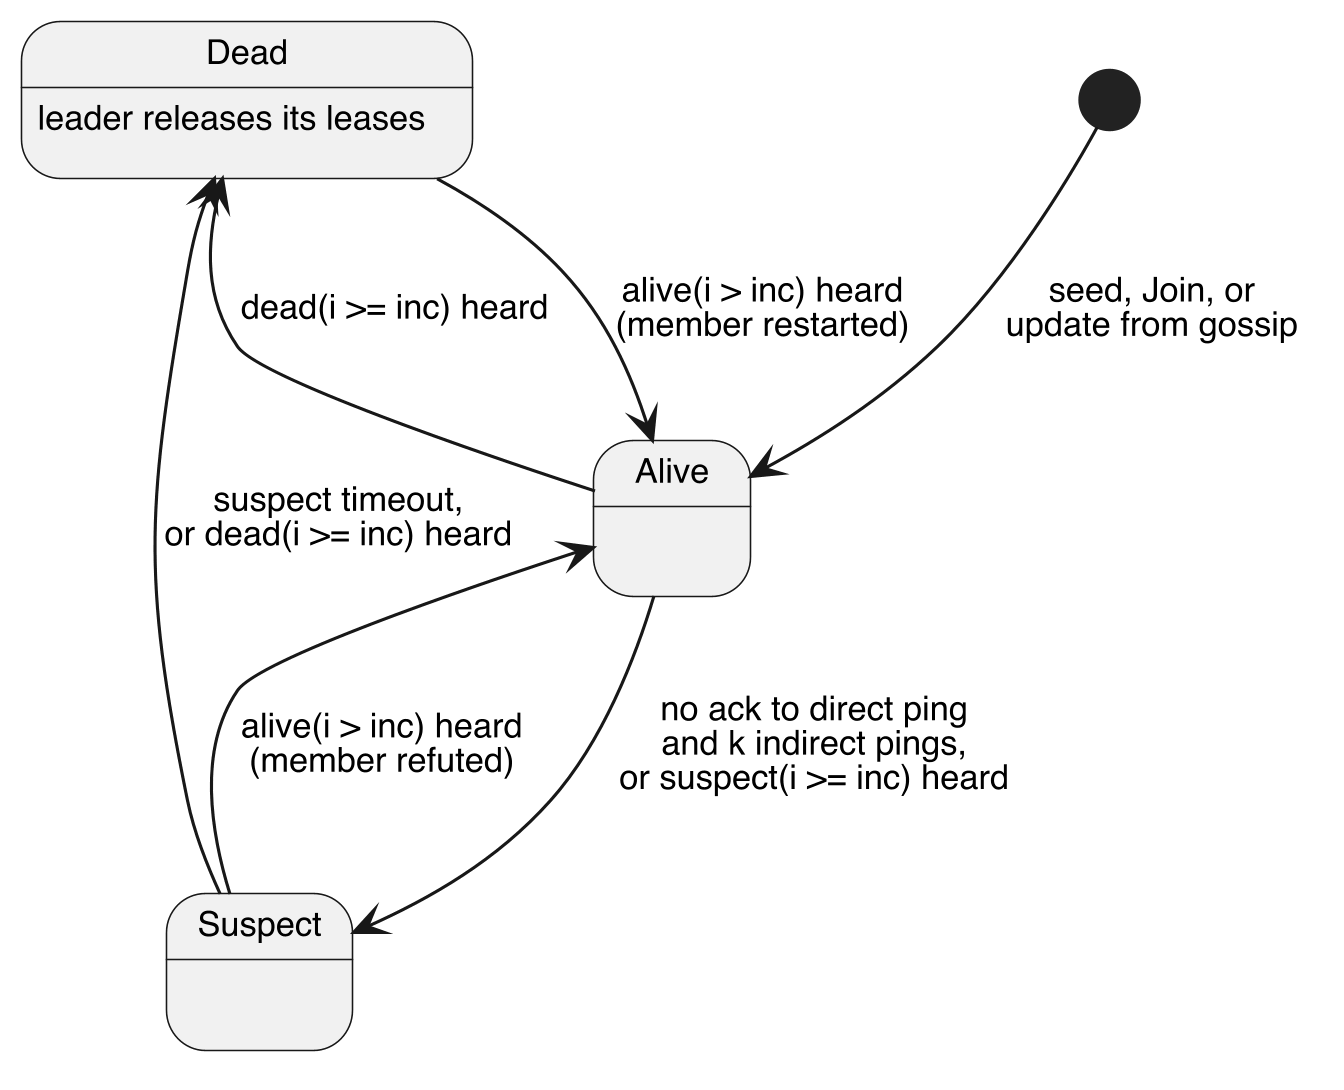
\includegraphics[width=0.9\columnwidth]{d6-swim-state.png}
\caption{What one SWIM member believes about another (design diagram D6). Updates carry an incarnation number $i$; \textit{inc} is the incarnation currently known for the member.}
\label{fig:swim-state}
\end{figure}

\subsection{Architecture}
\label{sec:architecture}

Fig.~\ref{fig:use-case} summarizes what each actor can do. A \emph{client} submits a job, follows its progress and retrieves the merged result. A \emph{volunteer} registers with its token and its resources, requests work and returns results. An \emph{operator} starts and stops the cluster, sets tokens, keys and timeouts, and watches the metrics.

Fig.~\ref{fig:deployment} shows the target deployment. Three coordinators run in three AWS availability zones, so that the loss of one zone still leaves a majority. Volunteers run on EC2 spot instances spread over the zones and on the team's laptops, and a Prometheus server scrapes the metrics of every coordinator. Each process is a single Go binary configured by environment variables, so the same topology also runs as local processes or with Docker Compose. Terraform files create the AWS deployment; all measurements in this report were taken on one machine.

The components interact over the five gRPC services of Section~\ref{sec:components}. Clients and volunteers talk only to the leader, and work always flows by pull: the leader opens connections to volunteers only for gossip probes. The coordinators talk to each other for election and replication, and all coordinators and volunteers form one SWIM group (Fig.~\ref{fig:swim-state}). Inside the leader, the coordinator server is the only component that changes the task table. It consults the scheduler for resource discovery, the lease policy, the verifier for voting and the membership view, and sends each resulting change through replication.

Each unit moves through the states of Fig.~\ref{fig:unit-state}. A unit is open while it still needs copies; each copy is leased to a different volunteer, whose result is then recorded; and the unit is accepted when two results agree. If every copy is back and no two agree, the leader asks for two more copies and the unit needs volunteers again. A lease that expires, or whose volunteer gossip declares dead, returns its copy without a result. Fig.~\ref{fig:failover} shows a leader crash: heartbeats stop, the highest remaining coordinator starts an election in a new term, wins with the acceptance of the third coordinator, catches up to the newest table and starts serving. Clients and volunteers find it by moving past the unreachable old leader and the follower that answers \texttt{FAILED\_PRECONDITION}, and volunteers then register again.

\begin{figure}[t]
  \centering
  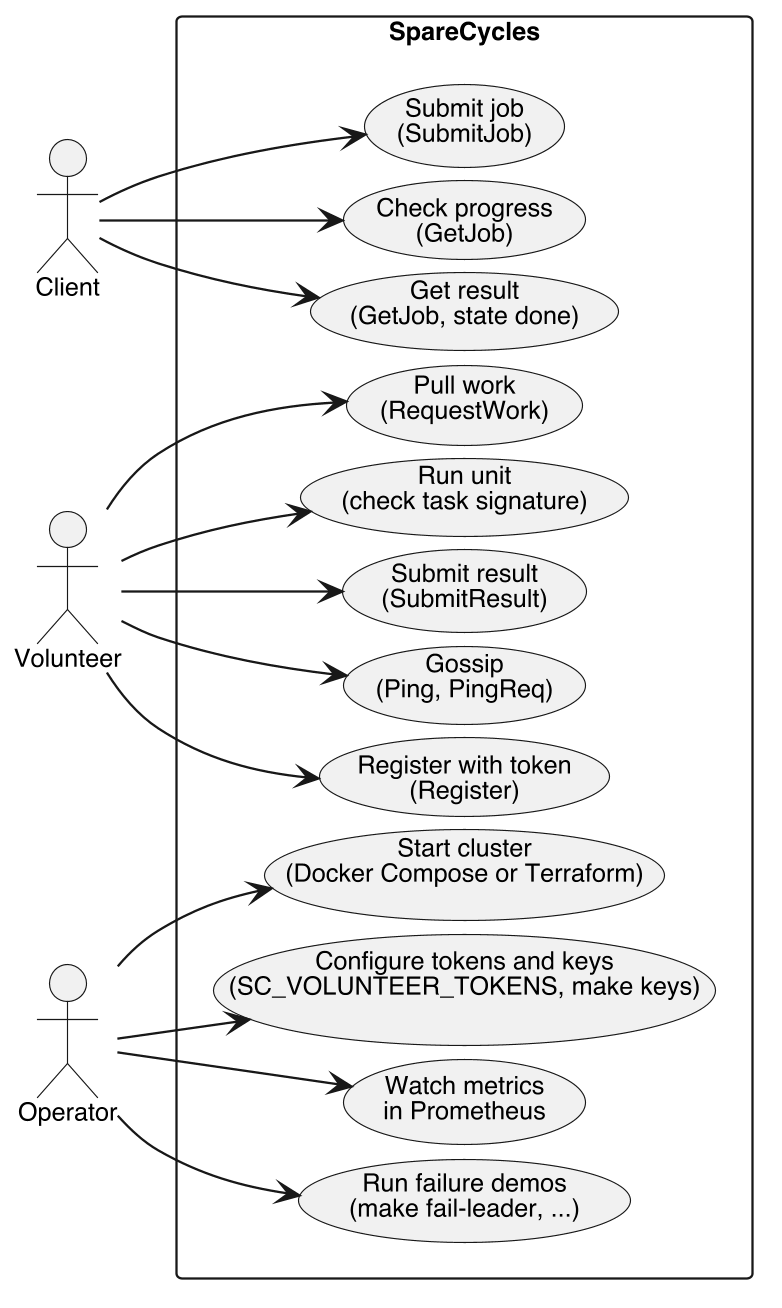
\includegraphics[width=0.8\columnwidth]{d1-use-case.png}
  \caption{Use cases of the three actors (design diagram D1). Clients and volunteers interact with the system only through gRPC calls to the leader and SWIM gossip, while the operator works outside the protocol through deployment, configuration, monitoring and the scripted failure demos.}
  \label{fig:use-case}
\end{figure}

\begin{figure*}[t]
  \centering
  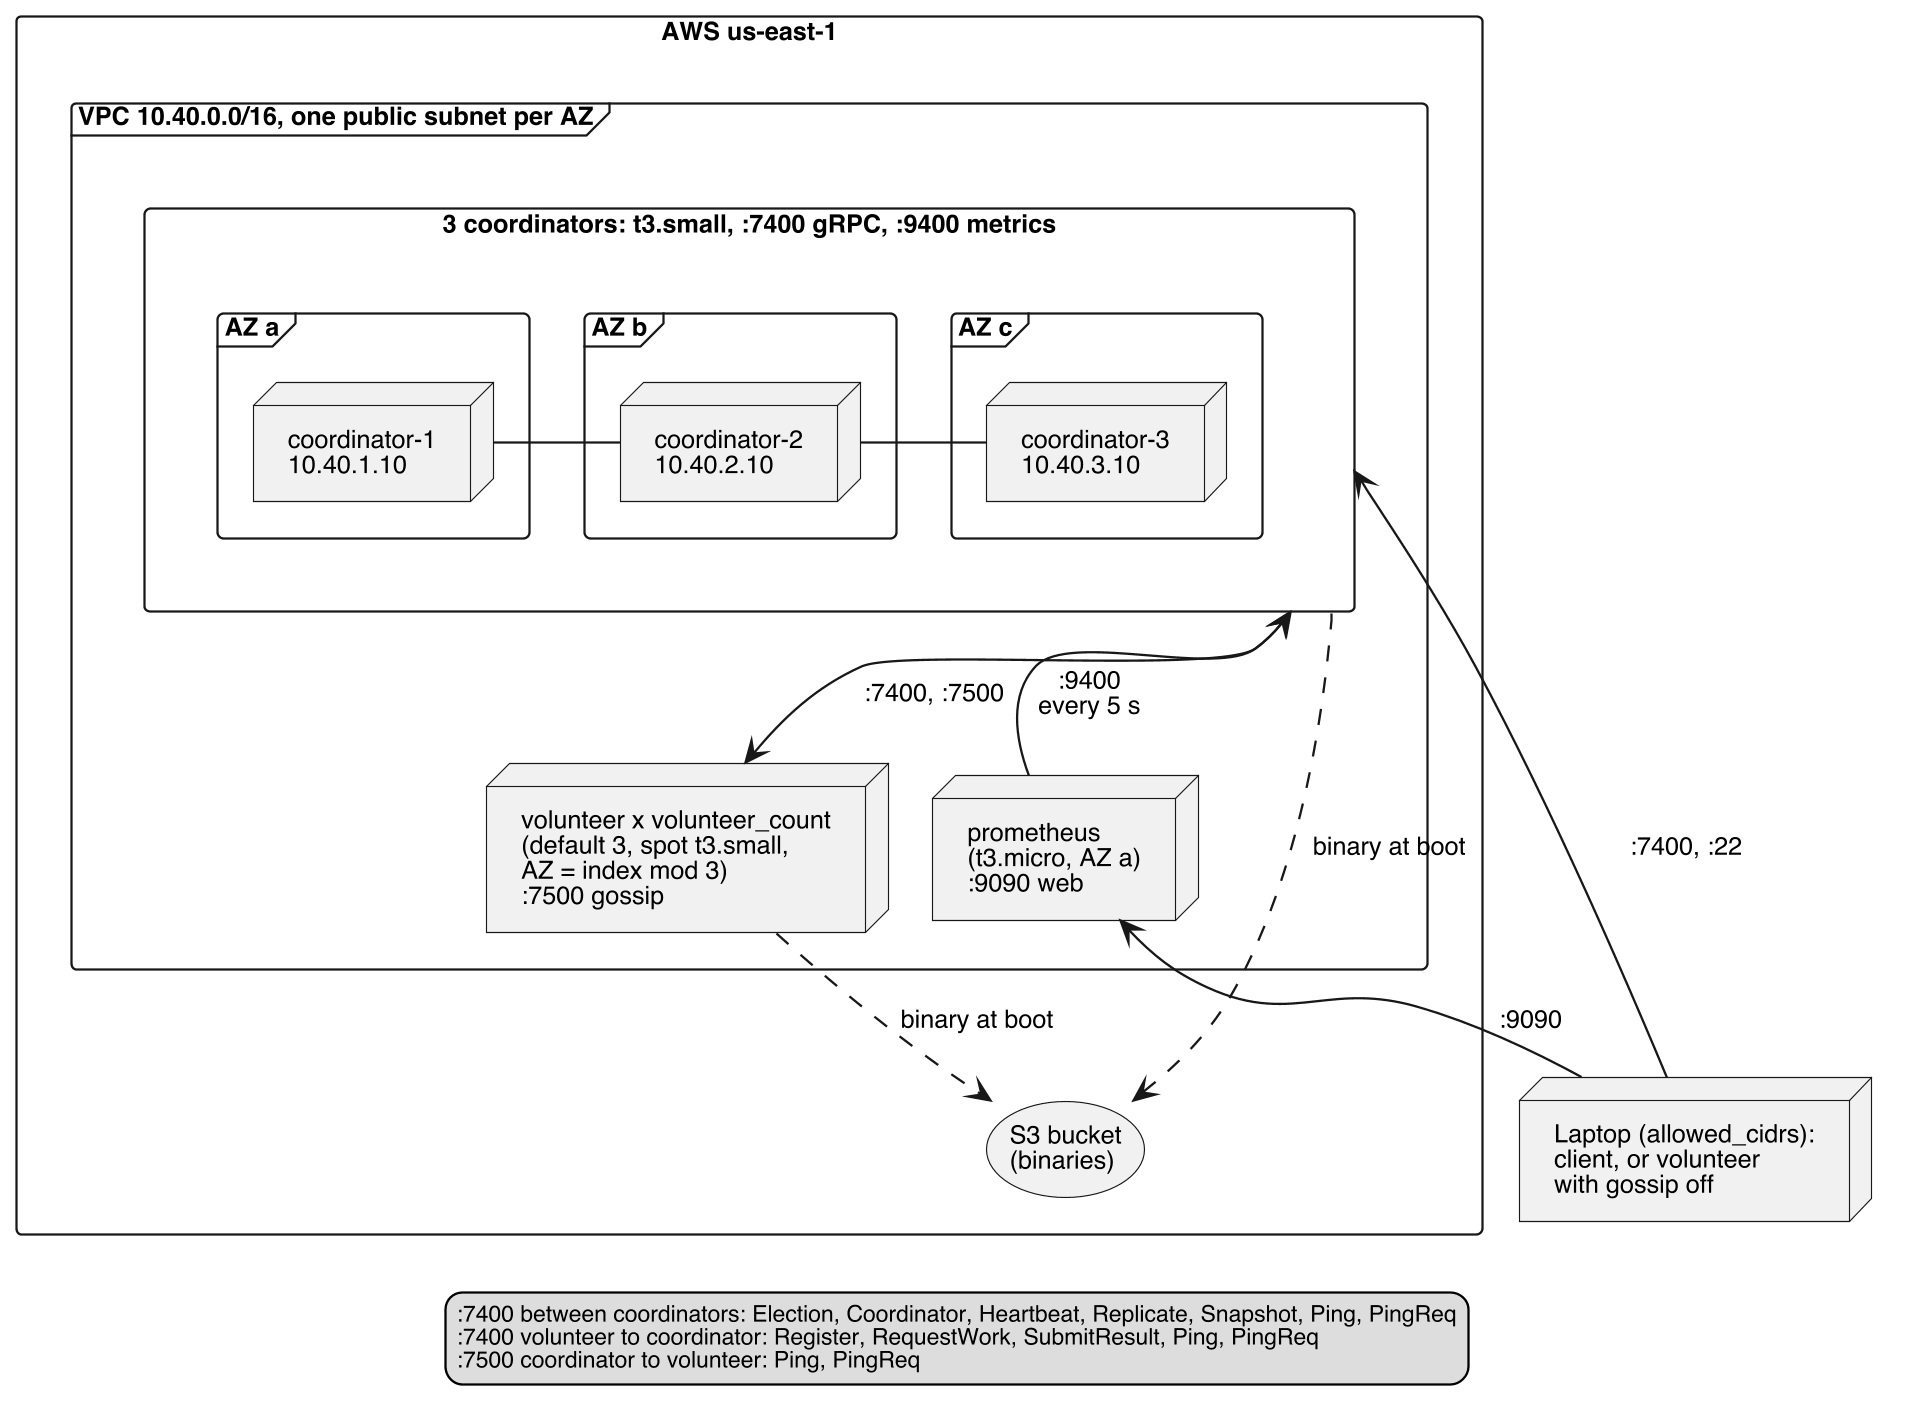
\includegraphics[width=0.78\textwidth]{d2-deployment.png}
  \caption{AWS deployment created by the Terraform configuration (design diagram D2). The three coordinators sit in separate availability zones with fixed private addresses, so the loss of one zone leaves a two-of-three majority, and the volunteers run on spot instances whose interruptions the lease and gossip mechanisms absorb.}
  \label{fig:deployment}
\end{figure*}

\begin{figure}[t]
  \centering
  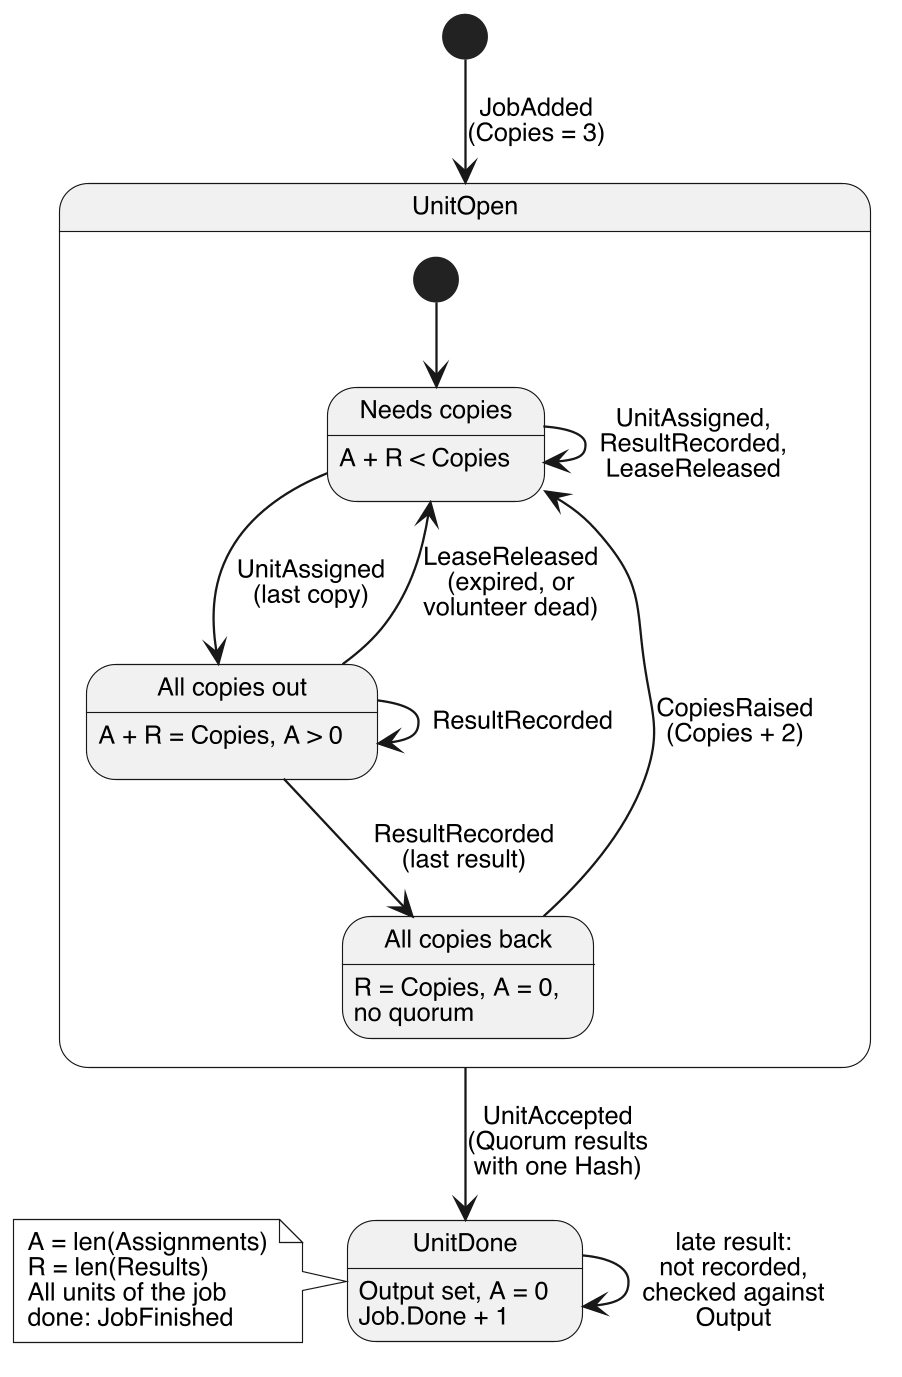
\includegraphics[width=0.85\columnwidth]{d4-unit-state.png}
  \caption{Life cycle of one work unit in the task table (design diagram D4). Each transition is a replicated task-table change; the table itself stores only \texttt{UnitOpen} and \texttt{UnitDone}, and the sub-states of an open unit follow from its number of leases and results.}
  \label{fig:unit-state}
\end{figure}

\begin{figure}[t]
  \centering
  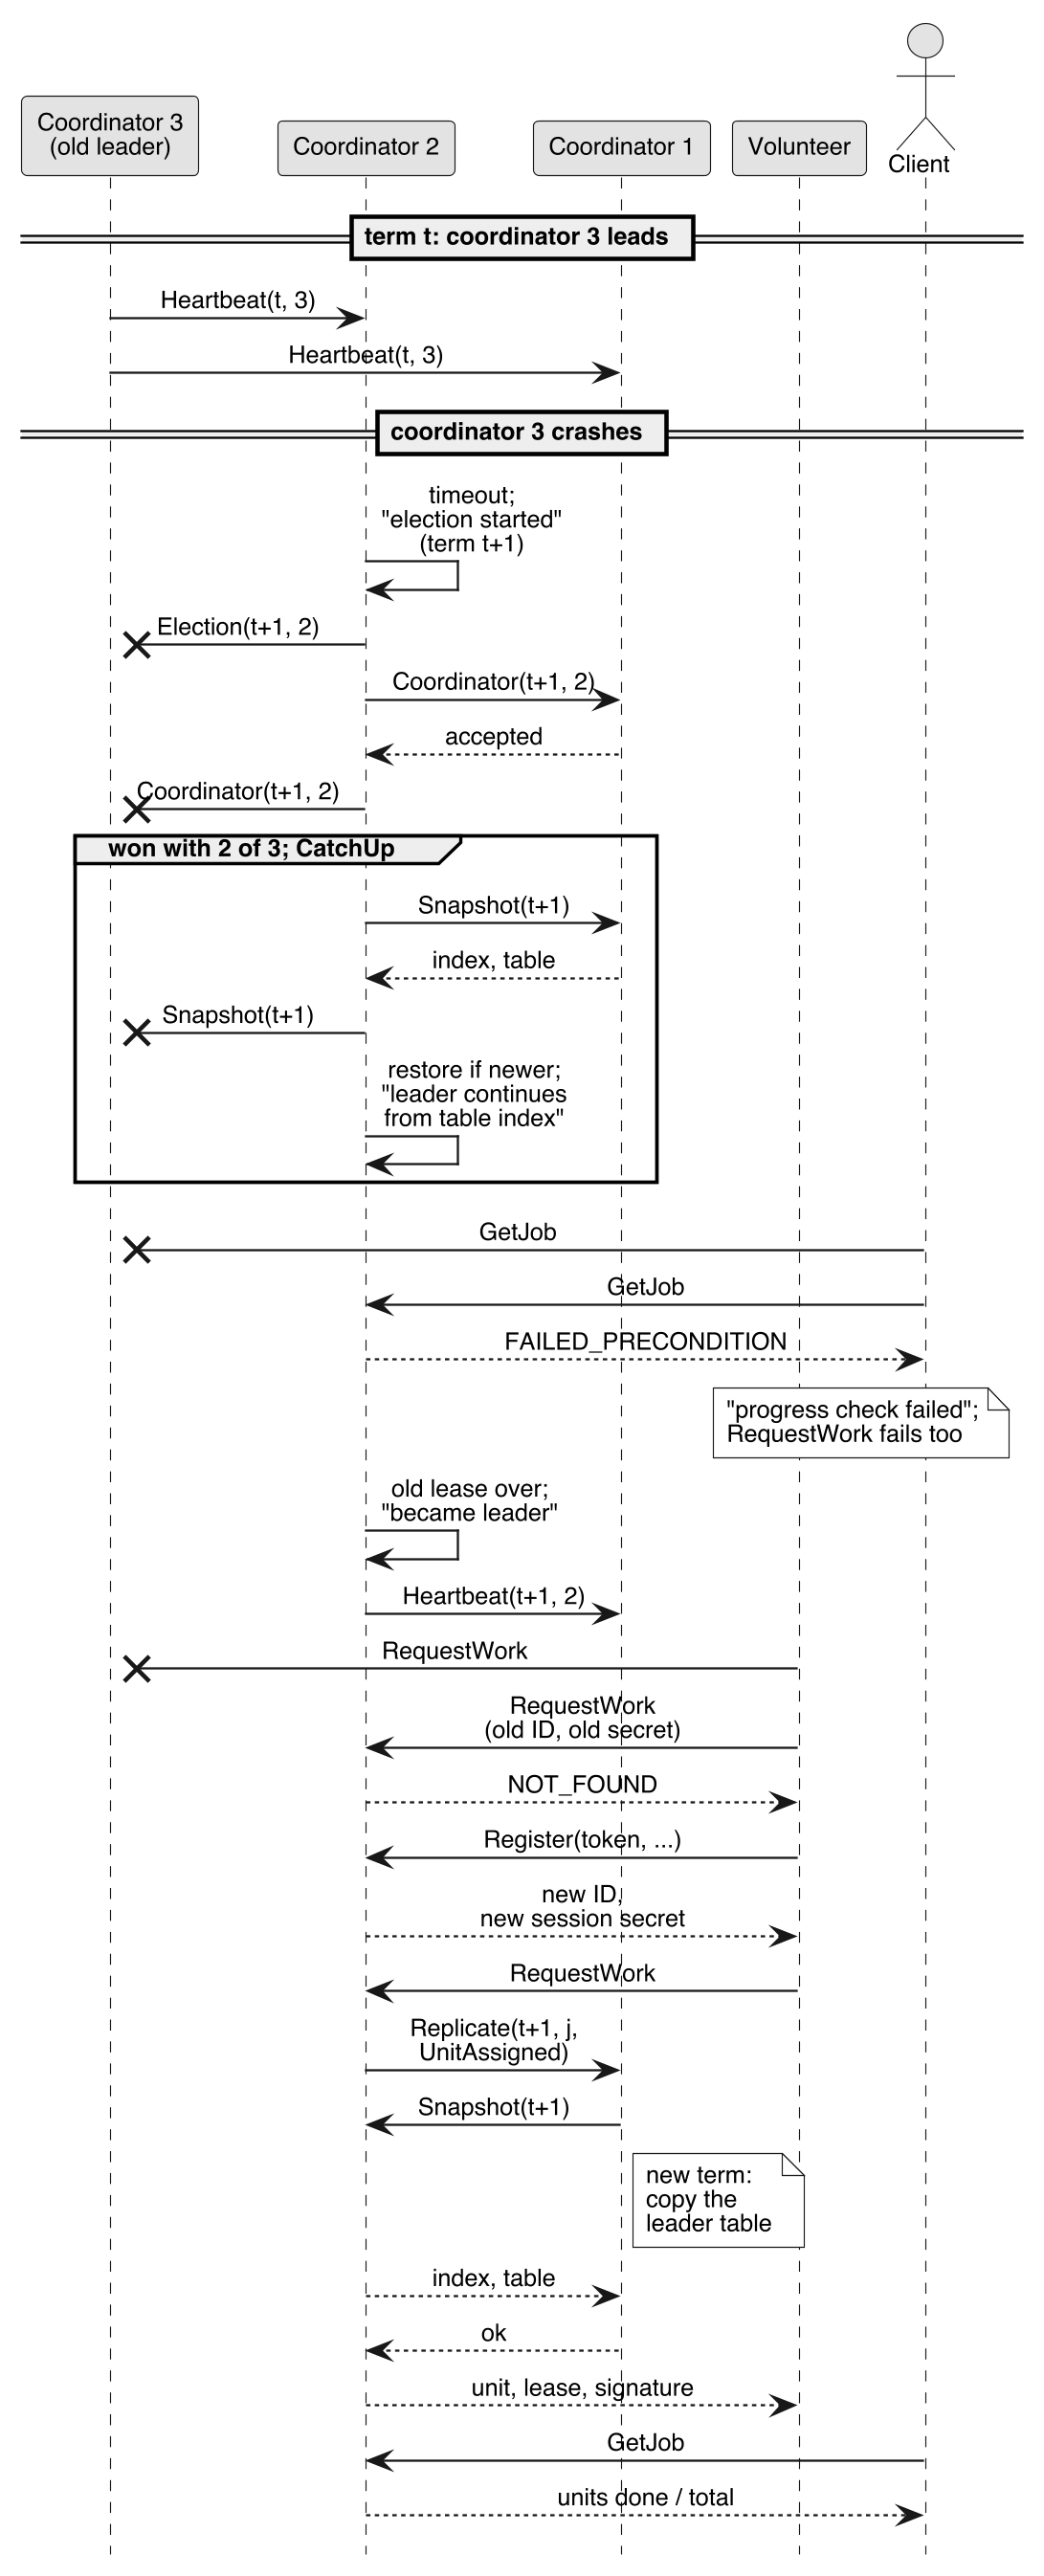
\includegraphics[width=0.72\columnwidth]{d5-failover-sequence.png}
  \caption{Failover after a crash of the leader (design diagram D5). Coordinator 2 wins a higher term with a majority, loads the newest table from the reachable coordinators before it acts, and the volunteer registers again because volunteer sessions are not replicated.}
  \label{fig:failover}
\end{figure}

Figure~\ref{fig:job-sequence} shows the life of one job. The leader splits the job into units and replicates the change before it confirms the job to the client. Volunteers pull units; each unit is given to three different volunteers, each with a lease and a signature. When two results agree, the leader accepts the unit, and when every unit is accepted it merges the outputs and records the final result.

\begin{figure*}[t]
\centering
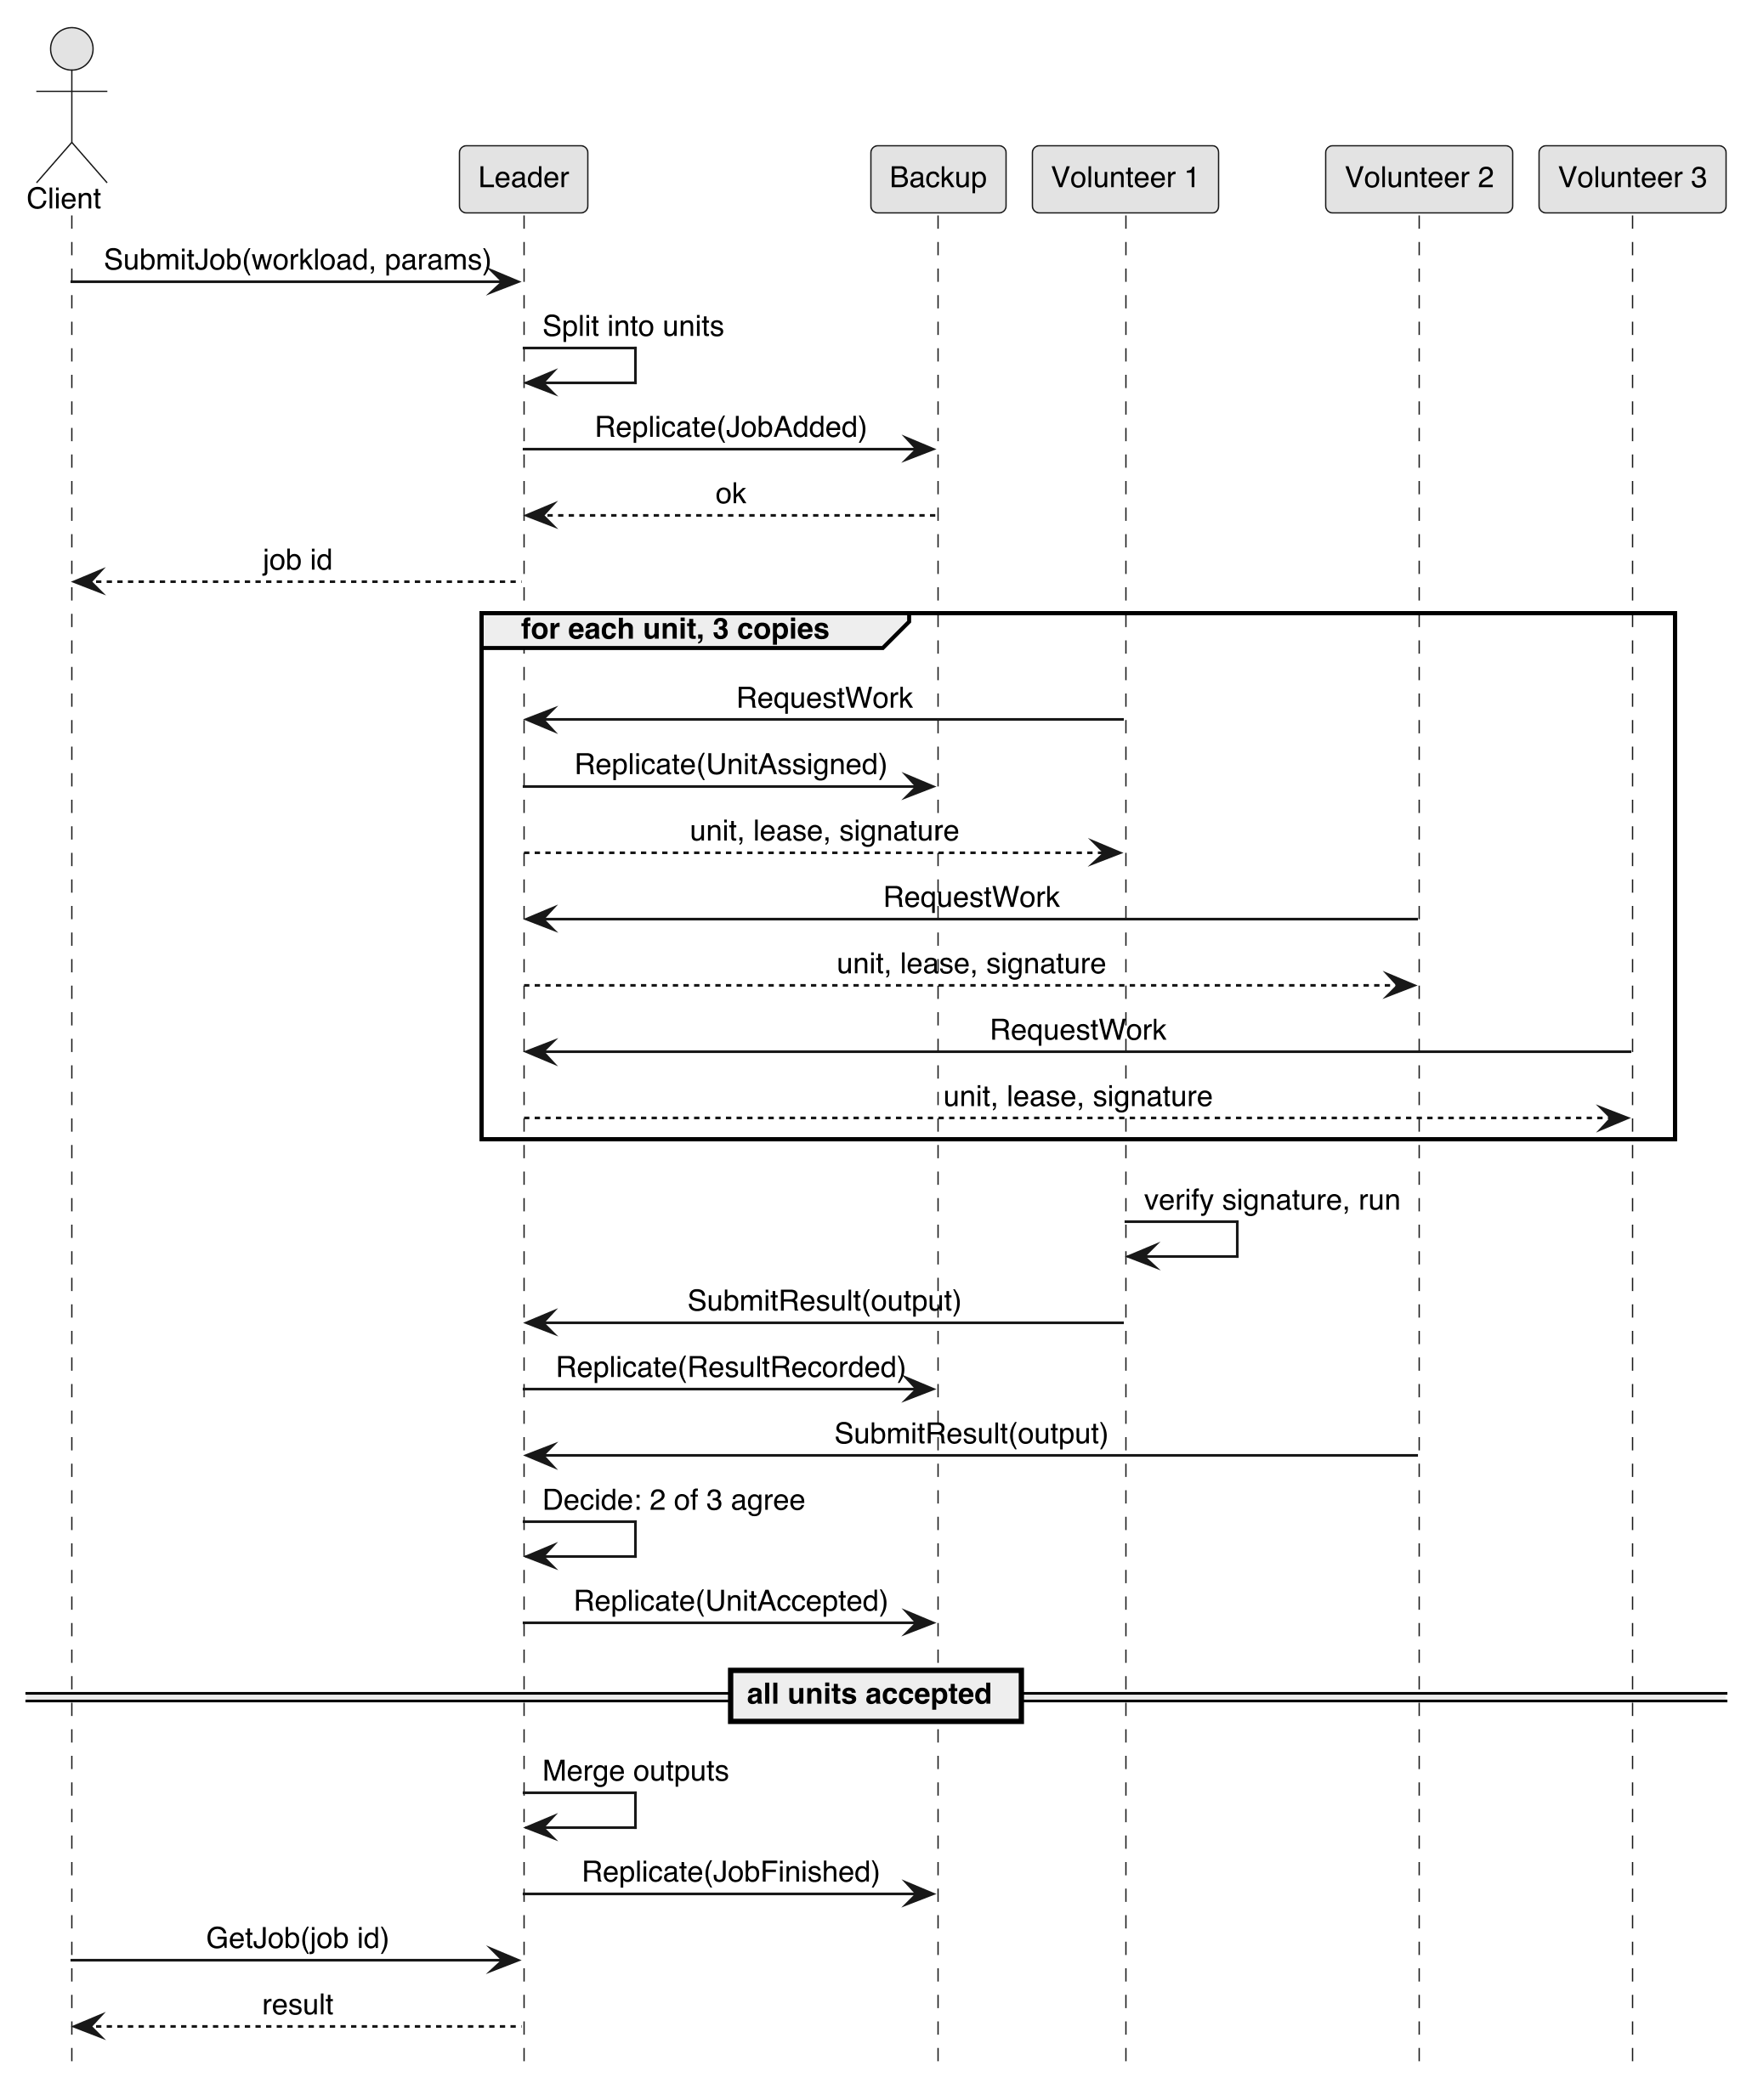
\includegraphics[width=0.8\textwidth]{d3-job-sequence.png}
\caption{One job from submission to result (design diagram D3). Every change to the task table is replicated to a backup before it is applied.}
\label{fig:job-sequence}
\end{figure*}

% Section 6. Owners: 6.1 each person for own algorithms; 6.2 split (see docs/report/outline.md).
\section{Evaluation of the Approach}
\label{sec:evaluation}

\subsection{Why the Approach Works}

\paragraph{Leases, majority voting, resource discovery} \todo{Tejas: intuition, correctness argument and complexity for each.}

\paragraph{Leader election, replication} \todo{Abhishek: intuition, correctness argument (one leader per term, no lost accepted work) and complexity for each.}

\paragraph{SWIM failure detection}
\emph{Intuition.} Instead of every member watching every other member, each member watches one other member per period, and asks a few others for a second opinion before it raises an alarm. News of the alarm then rides on traffic that already exists.

\emph{Correctness.} A failure detector is judged by completeness (every failure is eventually detected) and accuracy (live members are not declared failed). Completeness holds because the round-robin order guarantees that every live member probes a crashed member within a bounded number of periods, after which the suspicion becomes a death after the suspect timeout. Accuracy is probabilistic, as in any detector over an asynchronous network, but two mechanisms make false positives rare: a member is suspected only after its direct probe \emph{and} all $k$ indirect probes fail, and a wrongly suspected member refutes the suspicion before it becomes a death. Refutation is safe because updates are ordered by incarnation number: \textit{alive}$(i)$ overrides any state with a smaller incarnation, \textit{suspect}$(i)$ overrides \textit{alive}$(j)$ for $j \le i$, and \textit{dead}$(i)$ overrides both for $j \le i$. Every member applies the same rules, so members that hear the same updates in any order reach the same view. Two details matter in practice. A volunteer that registers again receives a new identifier, so an acknowledgement from a different identifier at the same address is treated as a failed probe of the old identifier. And a node starts with its incarnation set to the current Unix time, so that after a restart it overrules old reports of its own death.

\emph{Complexity.} With $n$ members, each member sends one probe per period, plus $k$ indirect requests only when a probe fails, so the load per member is $O(1)$ messages per period and the group load is $O(n)$. A message carries at most nine member records, so its size is also $O(1)$. An update is forwarded $3\lceil\log_2 n\rceil$ times and reaches the whole group in $O(\log n)$ periods. Each member stores $O(n)$ state. Detection takes at most $2n-1$ periods until some member probes the failed member, plus the suspect timeout; in expectation the first probe comes after a constant number of periods.

\paragraph{Tokens, session secrets and signed tasks}
\emph{Intuition.} The coordinator only talks to volunteers it knows, each request provably comes from the volunteer whose identifier it carries, and a volunteer only runs work that provably comes from a coordinator.

\emph{Correctness.} Ed25519 is existentially unforgeable under chosen-message attacks~\cite{bernstein2012ed25519}, so without the private key an attacker cannot produce a valid signature on any message the coordinator did not sign. Because the signed message is a length-prefixed encoding of the unit, workload, lease expiry and payload, the encoding is injective: two different tasks never yield the same message, so a valid signature for one task is useless for any other. Token comparison runs in constant time over every entry, which removes the timing side channel of an early-exit comparison.

Tokens alone are not enough. Gossip spreads every volunteer identifier to all members, so after registration an identifier proves nothing, and a malicious volunteer could otherwise submit results or request work in another volunteer's name, spoiling votes and lowering that volunteer's trust score. Registration therefore also returns a fresh 256-bit secret drawn from the operating system's random source, of which the leader keeps only the SHA-256 hash. Every later request must carry the secret, and the leader compares hashes in constant time. An attacker who knows only the identifier must guess the secret, with success probability $2^{-256}$ per attempt. The secret is leader-local and needs no replication: after a failover, volunteers are unknown to the new leader and register again, receiving new secrets. Without transport encryption, an attacker who can read network traffic can still copy a secret; this, like confidentiality of task data, is out of scope.

\emph{Complexity.} Signing and verifying cost $O(|p|)$ for a payload of size $|p|$, dominated by hashing, plus a constant number of curve operations. Checking a token against $m$ entries of length up to $L$ costs $O(mL)$, which is negligible because it happens once per registration. Checking a session secret costs one hash of 32 bytes and one constant-time comparison, $O(1)$ per request.

\subsection{How the System Handles the Main Requirements}

\paragraph{Fault tolerance}
SpareCycles tolerates three kinds of fault. A crashed volunteer is detected by gossip within seconds (2.4--2.9\,s with demonstration settings, Section~\ref{sec:scenario-volunteer}) and its work is released; if gossip cannot reach it, its lease expires instead. Each unit already runs on three different volunteers, and the leader never gives the same unit to the same volunteer twice, so with majority voting a single faulty or malicious volunteer is outvoted. \todo{Tejas: confirm with measurements once majority voting (\#7) is merged.} A crashed leader is to be replaced by election, after which the new leader continues from its replicated copy of the task table. \todo{Abhishek: describe and measure leader failover once \#13 and \#14 are merged.}

\paragraph{Performance, scalability} \todo{Tejas: refer to Section~\ref{sec:performance}.}

\paragraph{Consistency, concurrency} \todo{Abhishek.}

\paragraph{Security}
Unknown volunteers cannot register: in our tests a guessed token was rejected and counted, while valid tokens were logged by name. A registered volunteer cannot act under another volunteer's identifier: in our tests all four forged requests, with no secret or with the attacker's own secret, were rejected, nothing was recorded, and the victim's genuine result still completed the job. A volunteer configured with the wrong public key found a bad signature on its first task, ran nothing and stopped; gossip then declared it dead and the leader moved its unit to an honest volunteer, so the job still finished (Section~\ref{sec:testing}). With no tokens or keys configured, the system stays open so that it can be tried immediately, and each process logs which mode is active.

% Section 7. Owners: 7.1 and 7.3 Kushagra; diagrams I1 Kushagra, I2 Abhishek, I3 Tejas.
\section{Implementation Details}
\label{sec:implementation}

\subsection{Architectural Style}
SpareCycles combines three architectural styles. At the system level it is a \emph{master--worker} system with \emph{pull-based} assignment: volunteers ask the leader for work, so a volunteer behind a home router needs no inbound connection for its main task, and the leader never has to track which volunteers are idle. The coordinator tier is a \emph{replicated state machine} in a primary--backup arrangement: the task table changes only through a small set of change records (job added, unit assigned, lease released, result recorded, copies raised, unit accepted, job finished), and applying the same records in the same order yields the same table on every coordinator. Inside each process, the code follows a \emph{ports-and-adapters} style: the coordinator depends only on small interfaces, one per algorithm, and each algorithm is an adapter behind its interface (Fig.~\ref{fig:classes}).

The last choice shaped how the team worked. We first built a complete system in which every algorithm was a trivial stub (for example, a leader that never changes and leases that never expire) and ran it end to end. Each team member then replaced one stub at a time behind a stable interface, with its own tests, without editing the code of the others.

\begin{figure*}[t]
\centering
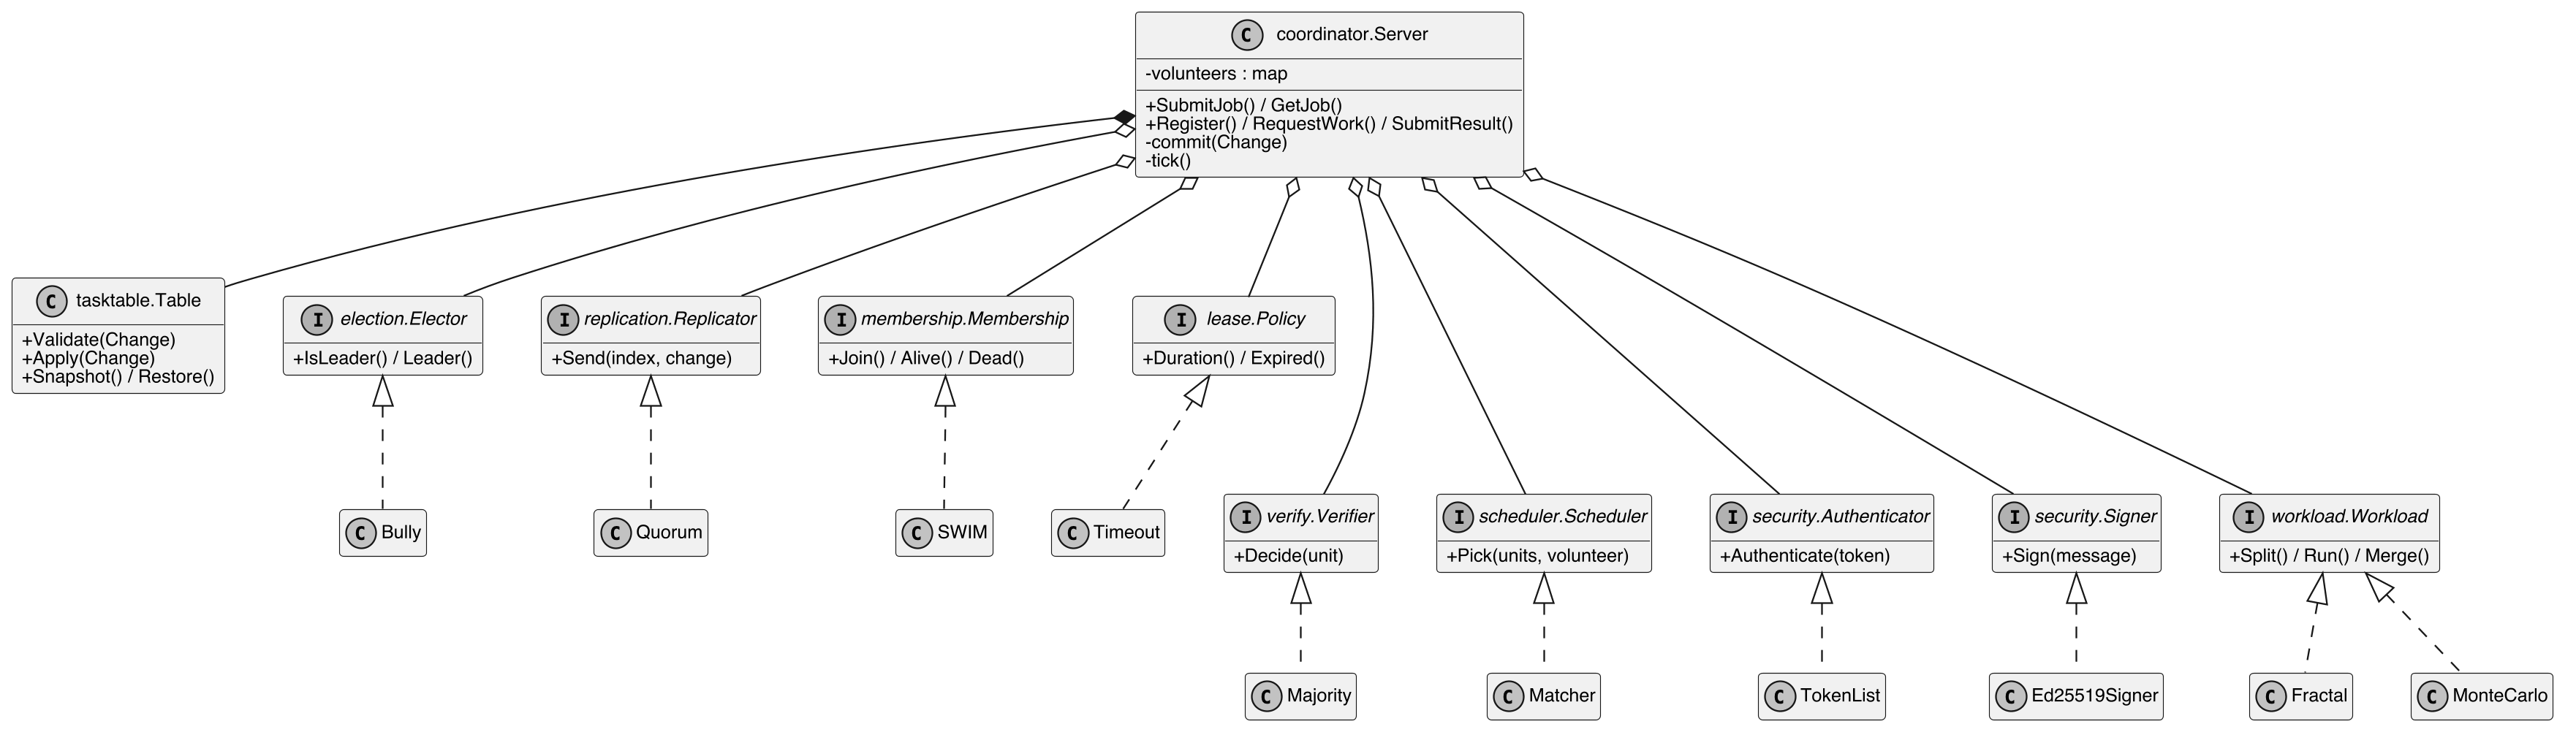
\includegraphics[width=\textwidth]{i1-coordinator-classes.png}
\caption{The coordinator and the interfaces of its parts (implementation diagram I1), with the implementations that the coordinator binary uses. The first stubs remain in each package for tests.}
\label{fig:classes}
\end{figure*}

Two rules keep the replicated state machine correct. Applying a change is deterministic: anything that varies, such as identifiers or lease expiry times, is computed by the leader and stored in the change itself. And every change is validated before it is replicated, under a single mutex that orders all changes, so a backup never receives a change that the leader would then reject.

\todo{Abhishek: implementation diagram I2 (component diagram of the Go packages). Tejas: implementation diagram I3 (object diagram of the task table during a job).}

\subsection{Software Components and Their Interaction}
\label{sec:components}
The system is written in Go and consists of three main programs (coordinator, volunteer and client) and two tools (a key generator and a load generator). All network communication uses gRPC with Protocol Buffers. One contract file defines five services:

\begin{itemize}
\item \texttt{ClientService} (client to leader): submit a job, read its progress and result.
\item \texttt{VolunteerService} (volunteer to leader): register, request work, submit a result.
\item \texttt{ElectionService} (coordinator to coordinator): election, coordinator announcement, heartbeat.
\item \texttt{ReplicationService} (leader to backups): replicate one change, send a snapshot.
\item \texttt{GossipService} (any member to any member): ping and indirect ping.
\end{itemize}

Only the leader serves client and volunteer requests; a follower answers with the gRPC status \texttt{FAILED\_PRECONDITION}. Clients and volunteers hold one connection to every coordinator and send each call to the coordinator that answered last, moving on to the next one when the answer is \texttt{FAILED\_PRECONDITION} or \texttt{UNAVAILABLE}. This one rule makes leader failover transparent to them. Volunteers run their own small gRPC server for gossip only.

Every setting is an environment variable with a default that works on one machine, so the system runs immediately after a clone. Each coordinator exports Prometheus metrics for every main event, such as units accepted, leases released after a death, gossip members by state and registrations rejected. Tests run complete jobs inside one process over in-memory gRPC connections, and the continuous integration pipeline runs every test with the Go race detector on each change.

% Section 8. Owners: 8.1 Tejas; 8.2 one scenario each (Kushagra, Tejas, Abhishek).
\section{Demonstration of Example System Runs}
\label{sec:demo}

Each scenario runs with one command from a fresh clone (\texttt{make fail-volunteer}, \texttt{make fail-faulty}, \texttt{make fail-leader}). The scripts start a local cluster, inject the failure, keep every log, and print \texttt{PASS} or \texttt{FAIL}.

\subsection{Success Scenario}
\todo{Tejas: one job end to end (TC-01): client progress and the resulting fractal image as screenshots.}

\subsection{Failure Scenario 1: A Volunteer Crashes}
\label{sec:scenario-volunteer}
One coordinator and two volunteers run a job of 256 units, each unit on a single volunteer so that only gossip can rescue a lost unit. Gossip uses a 300\,ms period, a 150\,ms probe timeout and a 2\,s suspect timeout. Once volunteer~A has returned five results, it is killed with \texttt{kill -9}, which gives it no chance to say goodbye. Fig.~\ref{fig:volunteer-crash} shows the terminal output of the run, including the relevant lines of the coordinator log.

\begin{figure*}[t]
\centering
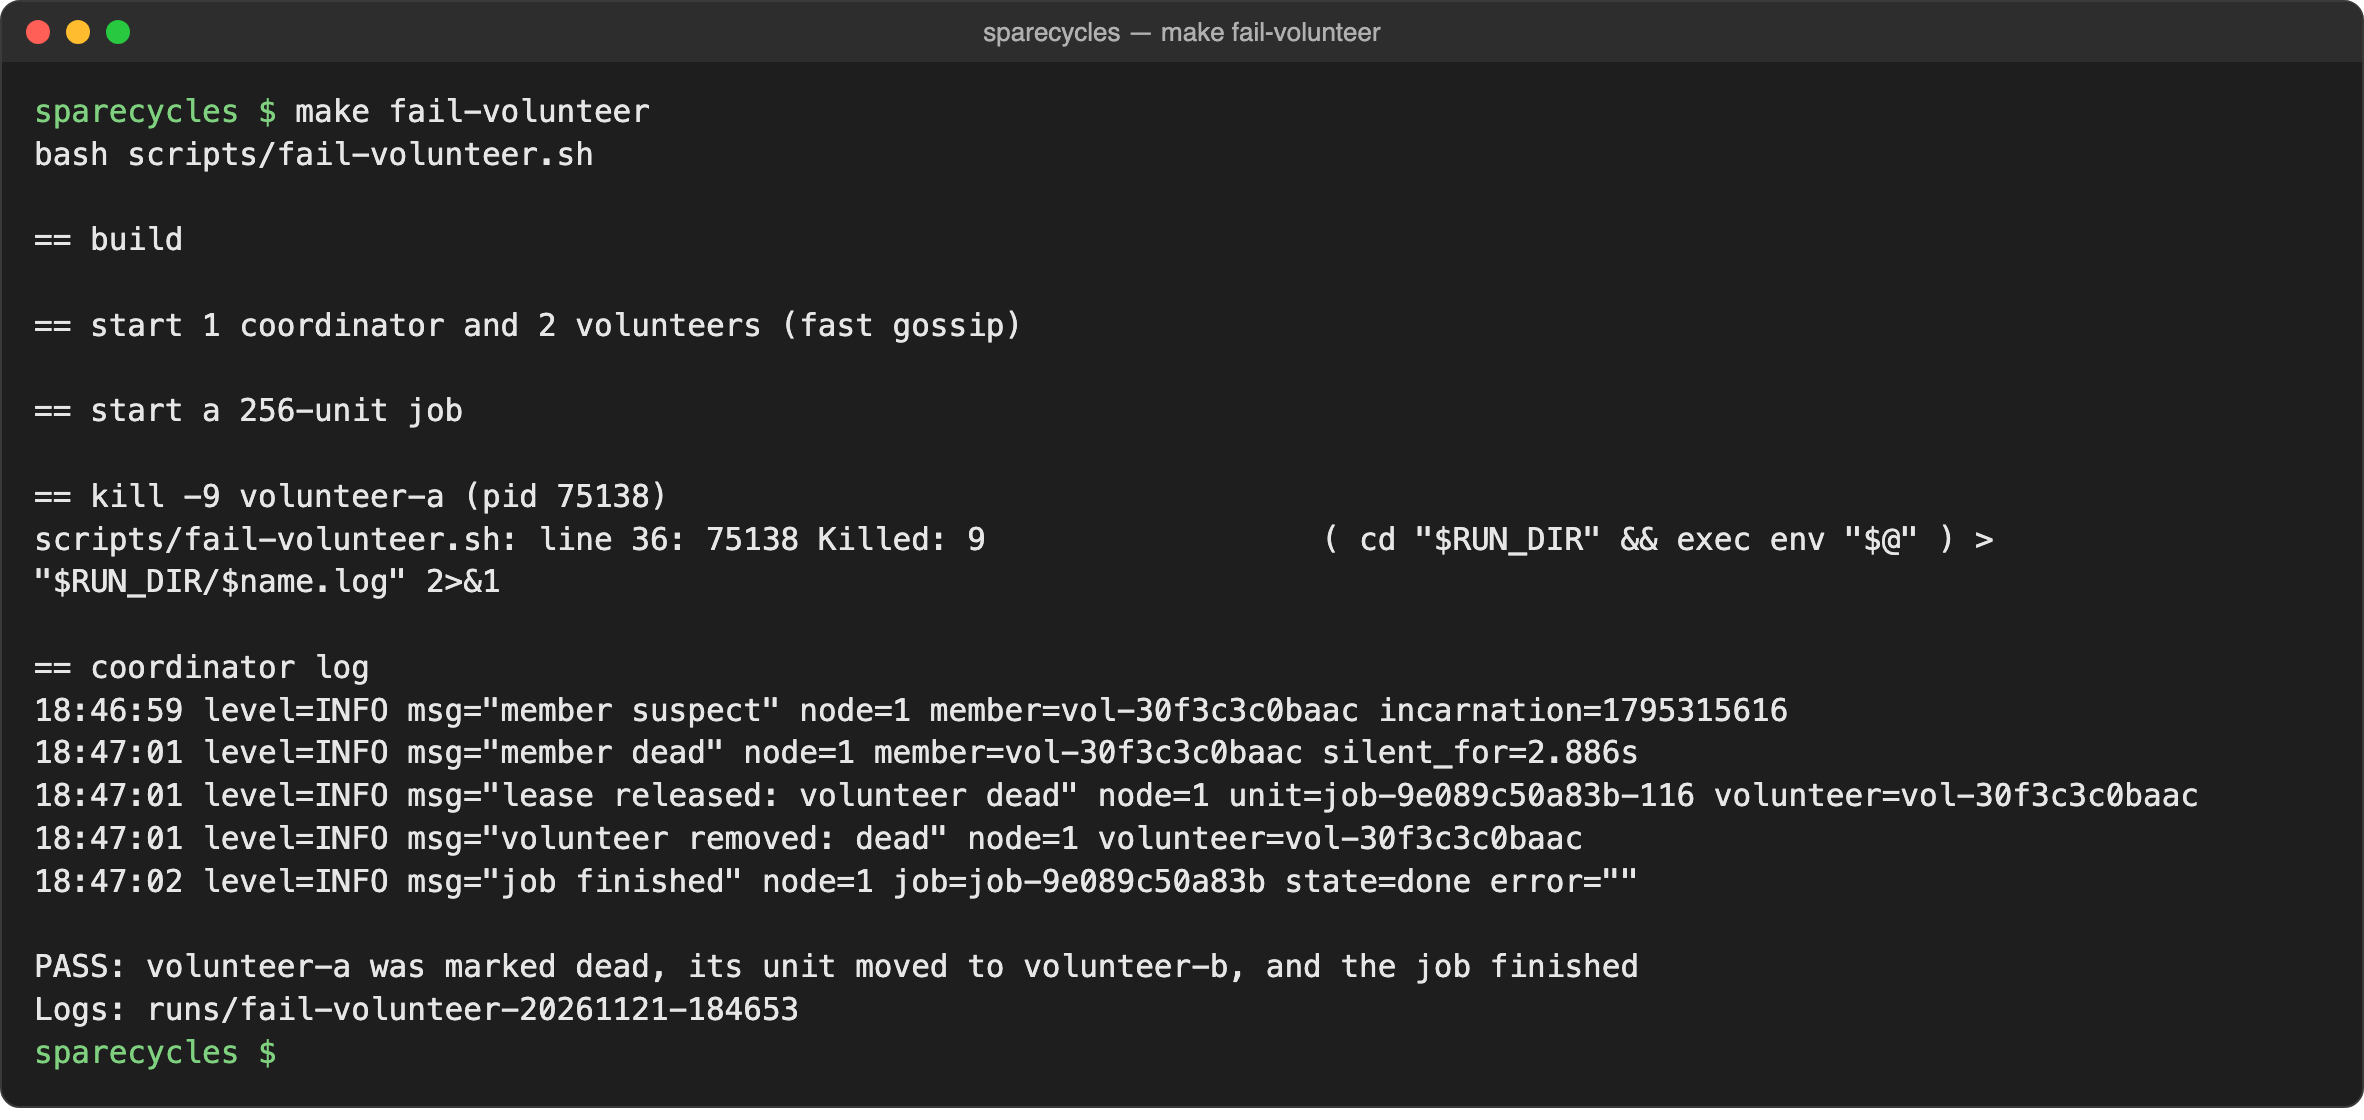
\includegraphics[width=0.9\textwidth]{s2-volunteer-crash.png}
\caption{Terminal output of \texttt{make fail-volunteer}: volunteer~A is killed during a 256-unit job, and the script prints the coordinator log lines for suspicion, death, the released lease and the finished job.}
\label{fig:volunteer-crash}
\end{figure*}

The coordinator first suspected the volunteer at 18:46:59 and declared it dead two seconds later, 2.9\,s after its last contact with it. In the same second it released the lease on unit 116, which volunteer~B then completed, and the job finished one second later. Without gossip the unit would have waited for its full three-minute lease. The volunteer that crashed is also removed from the leader's list; had it been wrongly declared dead, its next request would be refused and it would register again under a new identifier.

\subsection{Failure Scenario 2: A Faulty Volunteer}
\todo{Tejas: after \#7 merges, run \texttt{make fail-faulty} (one volunteer with \texttt{SC\_FAULTY\_RATE=1.0} among three honest ones). Show the \texttt{wrong result} log lines and that the image matches the honest reference.}

\subsection{Failure Scenario 3: The Leader Crashes}
\todo{Abhishek: after \#13 and \#14 merge, run \texttt{make fail-leader}. Show the election, the new term, the table index the new leader continued from, and that the job finished.}

% Section 9. Owners: growth rates each person for own algorithms; 9.1 Abhishek; 9.2-9.3 Kushagra.
\section{Performance Analysis}
\label{sec:performance}

\subsection{Growth Rate of the Major Algorithms}
\emph{Leases.} Granting a lease is $O(1)$; the leader's expiry scan grows linearly with the open units and active leases, $O(U + A)$ per one-second tick, and each expired lease costs one replicated table change, independent of the number of volunteers.

\emph{Majority voting.} Computation grows linearly with the replication factor: each unit runs between $q$ and $r$ times (2 and 3 by default, 2.0 to 2.6 measured), plus two executions for every round without a majority. The leader's voting work is $O(r)$ per result, hence $O(r^2)$ per unit, which is negligible for $r = 3$.

\emph{Resource discovery.} Each work request costs the leader $O(Ur)$ to build the candidates from $U$ open units and $O(Uf)$ for the end-of-work check with $f$ active fast volunteers, while trust updates are $O(1)$. Because every unit needs at least $q$ requests, scheduling a backlog of $U$ units costs $O(U^2 r)$ in total when all of them are open at once; we did not measure this cost separately from the other per-request work.

\emph{Leader election.} An election with $n$ coordinators costs $n-1$ messages in the best case and $O(n^2)$ in the worst case, and in steady state the leader sends $n-1$ heartbeats per interval; neither cost depends on the number of volunteers, units or jobs. \emph{Replication.} Each change costs $n-1$ messages and one round trip to the fastest backup, and the number of changes grows linearly with the number of units times the copies per unit. A catch-up snapshot is linear in the size of the task table, so this is the only part of failover whose cost grows with the workload. Once a job finishes, the table keeps only its merged result and the hashes of its unit outputs, so the table grows by about one merged result per job (Section~\ref{sec:metrics}).

\subsection{Overall Result and Reflection}
SpareCycles meets its goals on a local cluster. All six algorithms and the security layer are written by the team, each failure scenario runs and passes with one command, and all 16 test cases pass. A crashed volunteer is declared dead within 3\,s with demonstration settings, a volunteer that returns only wrong results never changes the output and is blocked after its second wrong result, and a crashed leader is replaced 2.5\,s after the crash without losing accepted work. The price is throughput: with four volunteers, majority voting delivers 68\% of the baseline.

Looking back, the \emph{pull model} kept the leader simple, since it never tracks idle volunteers, but an idle volunteer polls every second, and with a single client the volunteers sat idle between jobs. \emph{Three copies with two of three agreeing} caught every wrong result in our runs, including those that arrived as late copies, yet every unit ran 2.0--2.6 times, which is the main cost of fault tolerance. \emph{Bully with terms and a leader lease} gave a predictable leader and a fast failover, but the textbook algorithm alone would have been unsafe; terms, majority acceptance and the lease were needed to make it so, and because Bully ignores how current a node's table is, a new leader must catch up before it acts. \emph{Primary-backup replication with one backup acknowledgement} tolerates the loss of any one coordinator at the latency of a single round trip, but it holds the commit lock during that round trip; since our load tests ran with one coordinator, their numbers do not include this cost. \emph{SWIM} paid off twice: it freed the work of a crashed volunteer in seconds instead of minutes, and after a failover it freed the units leased to the volunteers' old identifiers. Finally, the \emph{stub-first workflow} let three people work in parallel behind stable interfaces on a system that ran end to end from the start, and the end-to-end scripts found problems that unit tests had missed: the first run of the faulty-volunteer scenario failed because a faulty volunteer that always ran the third copy was never compared, which led to the checking of late copies, and a leader crash under sustained load on the Docker cluster showed that the task table grew without bound (Section~\ref{sec:metrics}).

\subsection{Metrics and Comparison with a Baseline}
\label{sec:metrics}
Every coordinator exports Prometheus metrics for its main events, including accepted units, jobs, gossip members by state, lease releases, wrong results, elections, failover time and replication time, together with the standard process metrics. Fig.~\ref{fig:prometheus} shows three of them during a five-minute run on the Docker Compose cluster of three coordinators and three volunteers, with two clients submitting jobs continuously. We killed one volunteer after 90\,s and the leader, node~3, 90\,s later. The three coordinators declared the volunteer dead 7.8 to 9.0\,s after their last contact with it, with the default gossip settings, and each then counted one live member less. Node~2 became leader 2.3\,s after the crash and continued from table index 26\,273, and the clients finished 447 jobs over the whole run. Throughput under the new leader recovered slowly, because a unit needs two matching copies and the second surviving volunteer registered with the new leader only about 18\,s after the takeover.

\begin{figure*}[t]
\centering
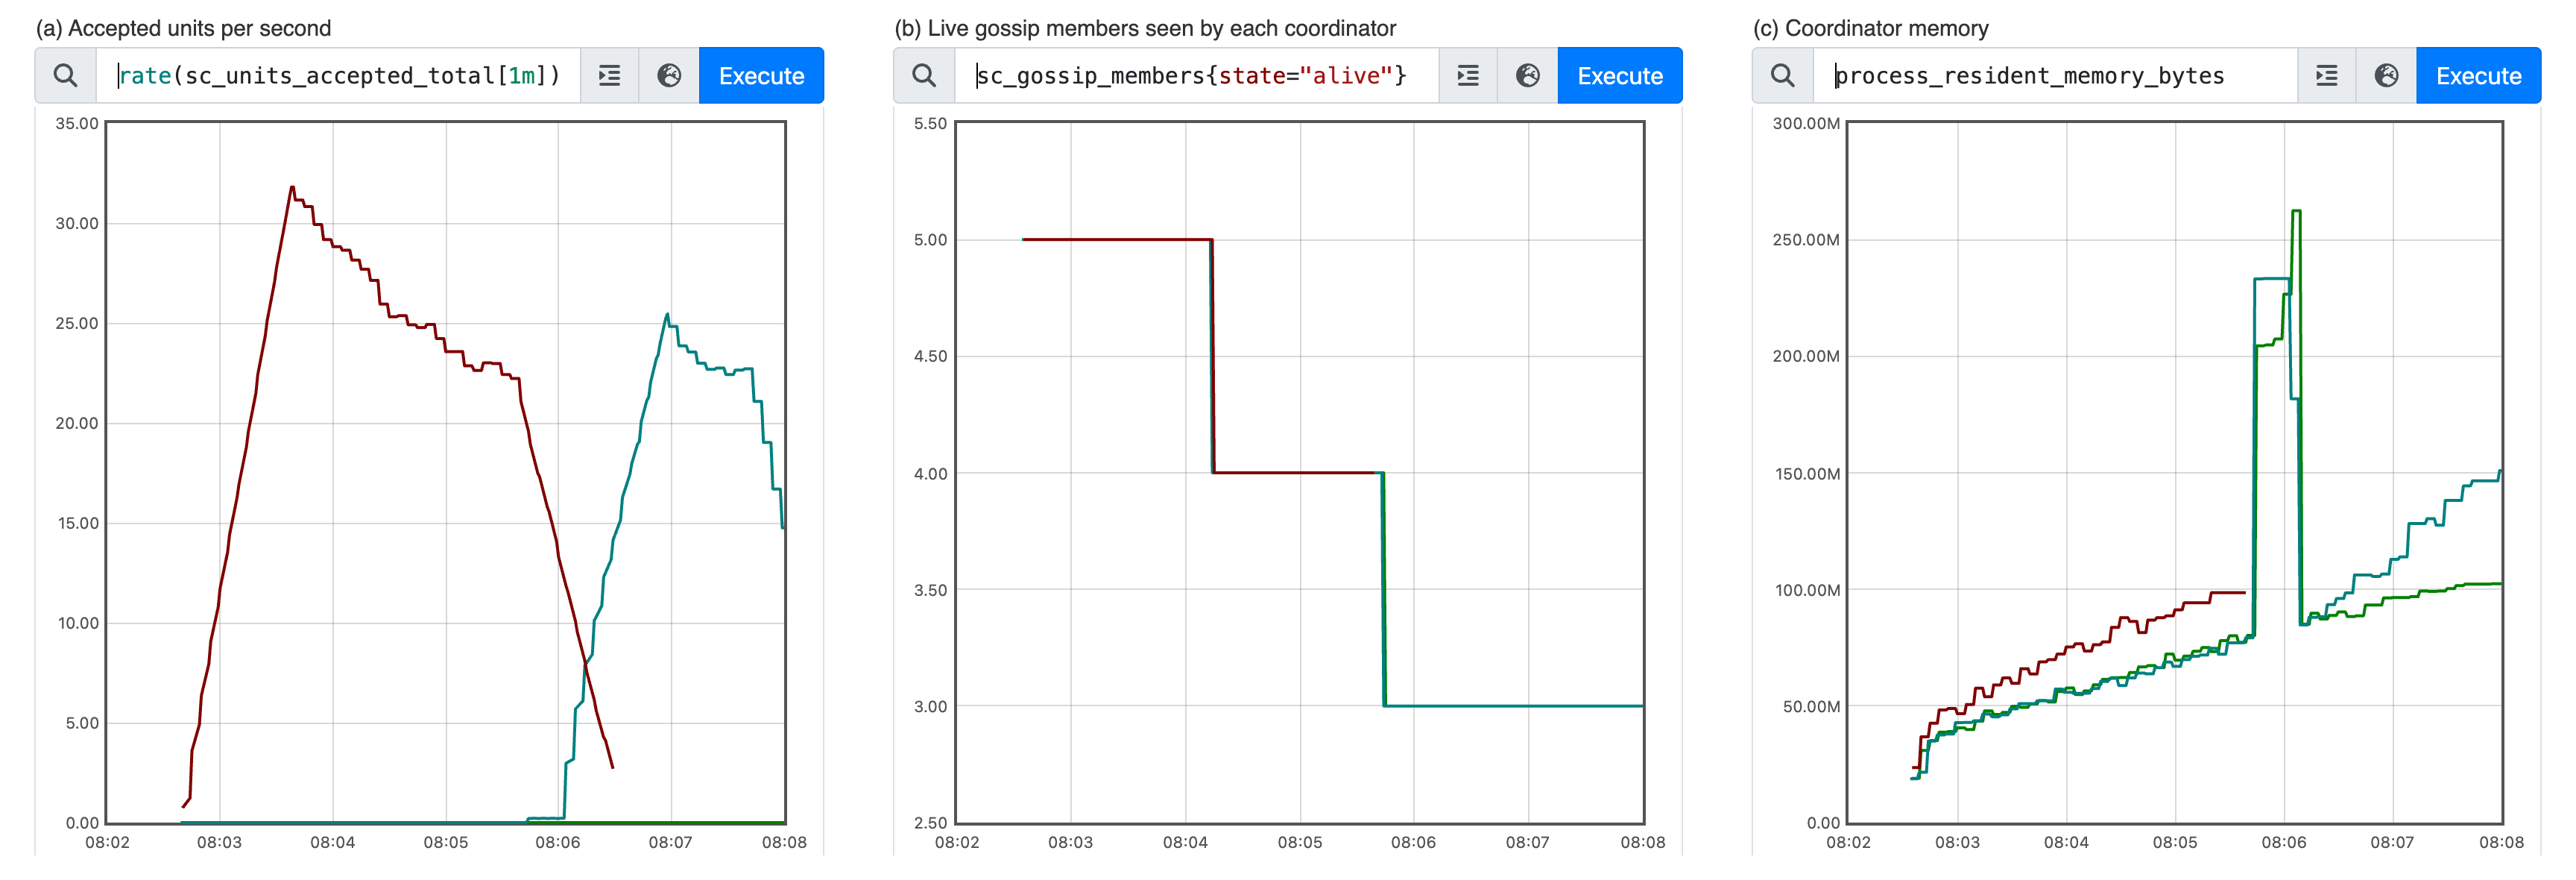
\includegraphics[width=\textwidth]{s5-prometheus.png}
\caption{Prometheus during five minutes of load on the Docker Compose cluster (times in UTC). A volunteer is killed at 08:04:08 and the leader, coordinator~3, at 08:05:38; the load stops at 08:07:38. Colors: coordinator~1 green, 2 teal, 3 red. (a) Accepted units per second, averaged over one minute, move from coordinator~3 to coordinator~2. (b) Each coordinator sees one live gossip member less after each crash. (c) Memory stays below 270\,MB, including the catch-up after the failover.}
\label{fig:prometheus}
\end{figure*}

The memory panel records a problem that this run found. In its first attempt, the task table kept every finished job with all its unit outputs and copies, 3 to 4\,MB for each fractal job, and each coordinator grew by 7 to 9\,MB/s to 1.2--1.6\,GB within three minutes. At the leader crash, Docker stopped both remaining coordinators for lack of memory. In a repeat with the crash after 80\,s, when each table held about 0.7\,GB, building, sending and loading the catch-up snapshot raised the two to 3.4 and 3.75\,GB; Docker stopped the new leader, and the last coordinator, without a majority, could not elect a leader. The local failure scenario (Section~\ref{sec:scenario-leader}) had passed because its table was small. The table now drops each unit's payload and copy outputs when the unit is accepted, and the accepted outputs when the job finishes, keeping only their hashes, which suffice to check late copies. With this change, the same run stayed at 80--100\,MB per coordinator after three minutes, and the catch-up peaked at 260\,MB. The merged result of each job, about 50\,kB for a fractal image, still stays in the table so that the client can fetch it; a long-running deployment would also need to remove finished jobs.

We measure throughput as accepted units per second and jobs per minute, and latency as the time from submitting a job to its result (mean and 95th percentile). To isolate the cost of fault tolerance, we compare two configurations of the same system on the same hardware: \emph{baseline}, in which each unit runs on one volunteer with no redundancy, and \emph{full}, in which each unit is sent to three different volunteers as majority voting requires. The baseline corresponds to a classic master--worker system without replication; the full configuration corresponds to BOINC-style redundant computing~\cite{anderson2004boinc}.

% Section 9.3 (part of 09-performance.tex). Owner: Kushagra. Data: results/load.csv, docs/test-results.md TC-07, TC-08, TC-11.
\subsection{Simulated Workloads}
A load generator submits eight fractal jobs of 64 units each (a $1024\times1024$ image in $128\times128$ tiles, 2000 iterations) against one coordinator. All processes run on one laptop with 10 cores (Apple silicon), started in the foreground from a terminal. At the time of measurement, the full configuration accepted the first returned result instead of waiting for a two-of-three majority; it therefore measures the cost of running three copies, which dominates the cost of voting. A repeated run differed by less than 0.2\%.

\paragraph{More volunteers}
With two clients submitting at the same time, we vary the number of volunteers (Table~\ref{tab:load}, Fig.~\ref{fig:load}). The baseline grows from 69 to 110 and 140 units per second, a factor of 2.0 for four volunteers. The shortfall from a factor of four has a clear cause: in this test a unit computes for only about 15\,ms, whereas the design targets units of about 60\,s, so the per-unit messages to the coordinator (a request, a result and two replicated table changes) are a large share of the cost. With realistic units this overhead would be negligible.

The full configuration behaves as a simple model predicts. With $N$ volunteers and three copies per unit, each unit occupies $\min(N,3)$ volunteers, so the useful throughput is about $N/\min(N,3)$ times that of a single volunteer. For $N=1$ and $N=2$ this means no gain over one volunteer, and indeed the full configuration delivers 68.2 and 69.2 units per second, the same as one baseline volunteer. With four volunteers it reaches 74.1 units per second, 53\% of the baseline, so fault tolerance costs 47\% of the throughput. For $N \ge 3$ the model predicts a share of one third, because every unit costs three executions however large the pool is; the measured share is higher because the baseline itself scales sublinearly in this test. This is the price of tolerating a malicious volunteer with replication. Two refinements could reduce it: adaptive replication, which BOINC applies to hosts with a good history, and early cancellation of the remaining copies once a majority agrees.

\begin{table}[t]
\centering
\caption{Throughput and job time with more volunteers (8 jobs, 512 units, 2 clients)}
\label{tab:load}
\begin{tabular}{@{}lrrrrr@{}}
\toprule
Mode & Vol. & Units/s & Jobs/min & Mean (s) & p95 (s) \\
\midrule
baseline & 1 & 69.1 & 64.8 & 1.75 & 2.55 \\
baseline & 2 & 109.6 & 102.8 & 1.12 & 2.14 \\
baseline & 4 & 139.6 & 130.8 & 0.89 & 1.64 \\
full & 1 & 68.2 & 63.9 & 1.76 & 2.45 \\
full & 2 & 69.2 & 64.9 & 1.75 & 2.55 \\
full & 4 & 74.1 & 69.5 & 1.63 & 2.15 \\
\bottomrule
\end{tabular}
\end{table}

\begin{figure}[t]
\centering
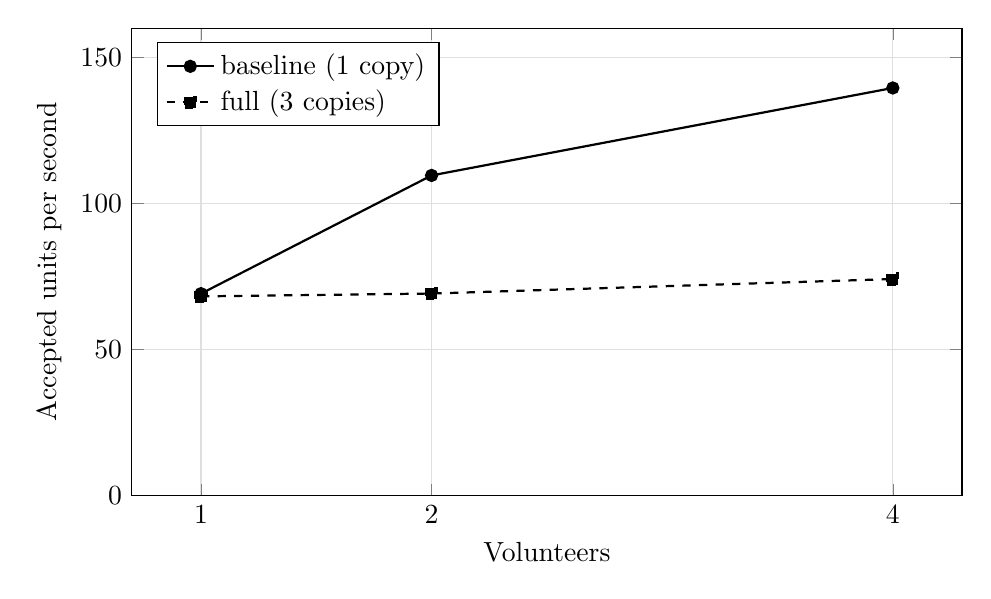
\begin{tikzpicture}
\begin{axis}[
  width=\columnwidth, height=0.62\columnwidth,
  xlabel={Volunteers}, ylabel={Accepted units per second},
  xtick={1,2,4}, ymin=0, ymax=160,
  legend pos=north west, legend cell align=left,
  grid=major, grid style={gray!25}]
\addplot[mark=*, thick] coordinates {(1,69.137) (2,109.607) (4,139.550)};
\addlegendentry{baseline (1 copy)}
\addplot[mark=square*, thick, dashed] coordinates {(1,68.207) (2,69.176) (4,74.142)};
\addlegendentry{full (3 copies)}
\end{axis}
\end{tikzpicture}
\caption{Throughput as volunteers are added, with 2 clients. Data: \texttt{results/load.csv}.}
\label{fig:load}
\end{figure}

\paragraph{More users}
With four volunteers in the full configuration, we vary the number of clients that submit jobs at the same time (Table~\ref{tab:clients}, Fig.~\ref{fig:clients}). With one client, the volunteers sit idle while a job is submitted, split and polled, so throughput is only 42.5 units per second. Two clients keep the volunteers busy, and throughput rises to 73.1. Beyond that it stays flat: the volunteers are the bottleneck, at about 75 units per second. Job time then grows with the number of clients, from a mean of 1.5\,s with one client to 4.7\,s with eight, as more jobs share the same volunteers; this is the expected queueing behavior. With eight clients, throughput falls slightly to 68.1 units per second, as more jobs and more polling compete for the single coordinator.

\begin{table}[t]
\centering
\caption{Throughput and job time with more clients (4 volunteers, full mode, 8 jobs)}
\label{tab:clients}
\begin{tabular}{@{}rrrrr@{}}
\toprule
Clients & Units/s & Jobs/min & Mean (s) & p95 (s) \\
\midrule
1 & 42.5 & 39.8 & 1.51 & 2.03 \\
2 & 73.1 & 68.5 & 1.64 & 2.25 \\
4 & 77.4 & 72.6 & 2.75 & 3.57 \\
8 & 68.1 & 63.9 & 4.66 & 7.52 \\
\bottomrule
\end{tabular}
\end{table}

\begin{figure}[t]
\centering
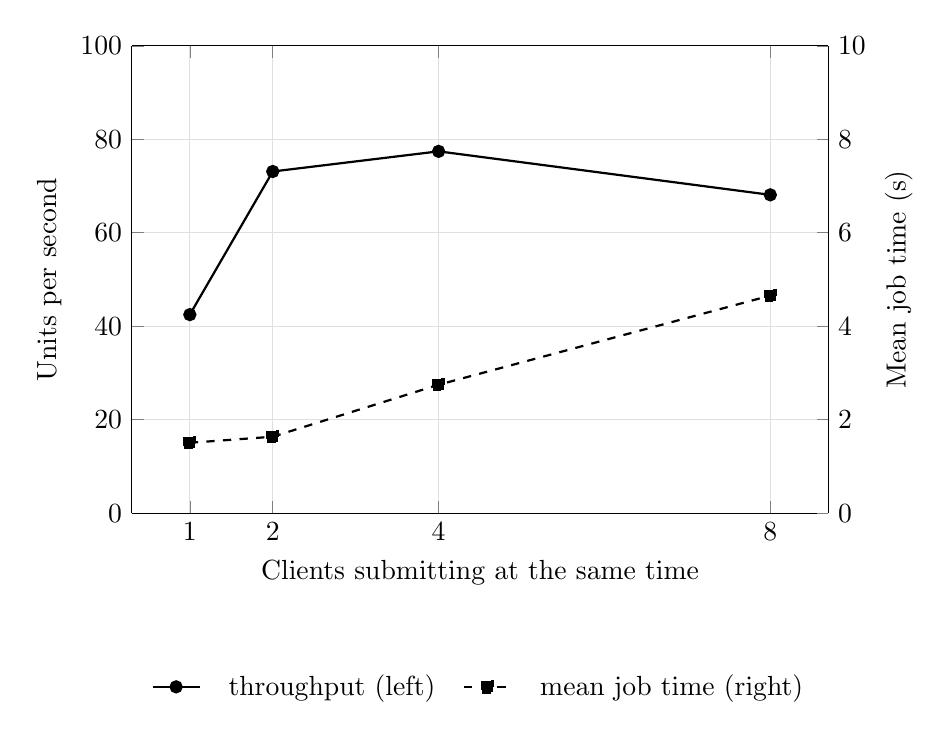
\begin{tikzpicture}
\begin{axis}[
  width=0.86\columnwidth, height=0.62\columnwidth,
  xlabel={Clients submitting at the same time}, ylabel={Units per second},
  xtick={1,2,4,8}, ymin=0, ymax=100,
  axis y line*=left,
  grid=major, grid style={gray!25}]
\addplot[mark=*, thick] coordinates {(1,42.489) (2,73.111) (4,77.420) (8,68.116)};
\end{axis}
\begin{axis}[
  width=0.86\columnwidth, height=0.62\columnwidth,
  xtick={1,2,4,8}, xticklabels={}, ymin=0, ymax=10,
  axis y line*=right, axis x line=none,
  ylabel={Mean job time (s)},
  legend style={at={(0.5,-0.32)}, anchor=north, legend columns=2, draw=none, column sep=8pt}]
\addlegendimage{mark=*, thick}
\addlegendentry{throughput (left)}
\addplot[mark=square*, thick, dashed] coordinates {(1,1.506) (2,1.637) (4,2.749) (8,4.656)};
\addlegendentry{mean job time (right)}
\end{axis}
\end{tikzpicture}
\caption{Throughput and job time as more users submit jobs (4 volunteers, full mode). Data: \texttt{results/load.csv}.}
\label{fig:clients}
\end{figure}


% Section 10. Owner: Tejas (each person adds own cases). Source: docs/test-results.md.
\section{Testing Results}
\label{sec:testing}

\todo{Tejas, about 0.6 page. Turn docs/test-results.md into a table of the test cases (ID, goal, method, result) and a short discussion. At least 5 cases; TC-01, TC-02 and TC-05 to TC-10 already have results. Add TC-03 (faulty volunteer) and TC-04 (leader crash) when \#7, \#13 and \#14 are merged. Mention that CI runs all automated tests with the race detector on every change.}

% Section 11. Owner: Abhishek.
\section{Conclusions}
\label{sec:conclusions}

\todo{Abhishek, about 0.4 page: what the project achieved, lessons learned (for example the stub-first workflow, the cost of replication, the gap between Bully and partition safety), and possible improvements (adaptive replication, early cancellation of copies, availability forecasting as in VECA, confidential computing).}


\bibliographystyle{IEEEtran}
\bibliography{references}

\end{document}
